% !TeX spellcheck = pl_PL
%%%%%%%%%%%%%%%%%%%%%%%%%%%%%%%%%%%%%%%%%%%
%                                        %
% Szablon pracy dyplomowej inzynierskiej %
% zgodny  z aktualnymi  przepisami  SZJK %
%                                        %
%%%%%%%%%%%%%%%%%%%%%%%%%%%%%%%%%%%%%%%%%%
%                                        %
%  (c) Krzysztof Simiński, 2018-2023     %
%                                        %
%%%%%%%%%%%%%%%%%%%%%%%%%%%%%%%%%%%%%%%%%%
%                                        %
% Najnowsza wersja szablonów jest        %
% podstępna pod adresem                  %
% github.com/ksiminski/polsl-aei-theses  %
%                                        %
%%%%%%%%%%%%%%%%%%%%%%%%%%%%%%%%%%%%%%%%%%
%
%
% Projekt LaTeXowy zapewnia odpowiednie formatowanie pracy,
% zgodnie z wymaganiami Systemu zapewniania jakości kształcenia.
% Proszę nie zmieniać ustawień formatowania (np. fontu,
% marginesów, wytłuszczeń, kursywy itd. ).
%
% Projekt można kompilować na kilka sposobów.
%
% 1. kompilacja pdfLaTeX
%
% pdflatex main
% bibtex   main
% pdflatex main
% pdflatex main
%
%
% 2. kompilacja XeLaTeX
%
% Kompilatacja przy użyciu XeLaTeXa różni się tym, że na stronie
% tytułowej używany jest font Calibri. Wymaga to jego uprzedniego
% zainstalowania.
%
% xelatex main
% bibtex  main
% xelatex main
% xelatex main
%
%
%%%%%%%%%%%%%%%%%%%%%%%%%%%%%%%%%%%%%%%%%%%%%%%%%%%%%
% W przypadku pytań, uwag, proszę pisać na adres:   %
%      krzysztof.siminski(małpa)polsl.pl            %
%%%%%%%%%%%%%%%%%%%%%%%%%%%%%%%%%%%%%%%%%%%%%%%%%%%%%
%
% Chcemy ulepszać szablony LaTeXowe prac dyplomowych.
% Wypełniając ankietę spod poniższego adresu pomogą
% Państwo nam to zrobić. Ankieta jest całkowicie
% anonimowa. Dziękujemy!


% https://docs.google.com/forms/d/e/1FAIpQLScyllVxNKzKFHfILDfdbwC-jvT8YL0RSTFs-s27UGw9CKn-fQ/viewform?usp=sf_link
%
%%%%%%%%%%%%%%%%%%%%%%%%%%%%%%%%%%%%%%%%%%%%%%%%%%%%%%%%%%%%%%%%%%%%%%%%%

%%%%%%%%%%%%%%%%%%%%%%%%%%%%%%%%%%%%%%%%%%%%%%%
%                                             %
% PERSONALIZACJA PRACY – DANE PRACY           %
%                                             %
%%%%%%%%%%%%%%%%%%%%%%%%%%%%%%%%%%%%%%%%%%%%%%%

% Proszę wpisać swoje dane w poniższych definicjach.

% TODO
% dane autora
\newcommand{\FirstNameAuthor}{Aleksandra}
\newcommand{\SurnameAuthor}{Kyc}
\newcommand{\IdAuthor}{296410}   % numer albumu  (bez $\langle$ i $\rangle$)

% drugi autor:
%\newcommand{\FirstNameCoauthor}{Imię}   % Jeżeli jest drugi autor, to tutaj należy podać imię.
%\newcommand{\SurnameCoauthor}{Nazwisko} % Jeżeli jest drugi autor, to tutaj należy podać nazwisko.
%\newcommand{\IdCoauthor}{$\langle$wpisać właściwy$\rangle$}  % numer albumu drugiego autora (bez $\langle$ i $\rangle$)
% Gdy nie ma drugiego autora, należy zostawić poniższe definicje puste, jak poniżej. Gdy jest drugi autor, należy zakomentować te linie.
\newcommand{\FirstNameCoauthor}{} % Jeżeli praca ma tylko jednego autora, to dane drugiego autora zostają puste.
\newcommand{\SurnameCoauthor}{}   % Jeżeli praca ma tylko jednego autora, to dane drugiego autora zostają puste.
\newcommand{\IdCoauthor}{}  % Jeżeli praca ma tylko jednego autora, to dane drugiego autora zostają puste.
%%%%%%%%%%

\newcommand{\Supervisor}{dr hab. inż., prof. PŚ Krzysztof Simiński}     % dane promotora (bez $\langle$ i $\rangle$)
\newcommand{\Title}{Aplikacja mobilna do nauki znaków kanji}           % tytuł pracy po polsku
\newcommand{\TitleAlt}{Mobile application for Kanji learning}                     % thesis title in English
\newcommand{\Program}{Informatyka}            % kierunek studiów  (bez $\langle$ i $\rangle$)
\newcommand{\Specialisation}{Grafika Komputerowa i Oprogramowanie}     % specjalność  (bez $\langle$ i $\rangle$)
\newcommand{\Departament}{Algorytmiki i Oprogramowania }        % katedra promotora  (bez $\langle$ i $\rangle$)

% Jeżeli został wyznaczony promotor pomocniczy lub opiekun, proszę go/ją wpisać ...
%\newcommand{\Consultant}{$\langle$stopień naukowy imię i nazwisko$\rangle$} % dane promotora pomocniczego, opiekuna (bez $\langle$ i $\rangle$)
% ... w przeciwnym razie proszę zostawić puste miejsce jak poniżej:
\newcommand{\Consultant}{} % brak promotowa pomocniczego / opiekuna

% koniec fragmentu do modyfikacji
%%%%%%%%%%%%%%%%%%%%%%%%%%%%%%%%%%%%%%%%%%


%%%%%%%%%%%%%%%%%%%%%%%%%%%%%%%%%%%%%%%%%%%%%%%
%                                             %
% KONIEC PERSONALIZACJI PRACY                 %
%                                             %
%%%%%%%%%%%%%%%%%%%%%%%%%%%%%%%%%%%%%%%%%%%%%%%

%%%%%%%%%%%%%%%%%%%%%%%%%%%%%%%%%%%%%%%%


%%%%%%%%%%%%%%%%%%%%%%%%%%%%%%%%%%%%%%%%%%%%%%%
%                                             %
% PROSZĘ NIE MODYFIKOWAĆ PONIŻSZYCH USTAWIEŃ! %
%                                             %k
%%%%%%%%%%%%%%%%%%%%%%%%%%%%%%%%%%%%%%%%%%%%%%%



\documentclass[a4paper,twoside,12pt]{book}
\usepackage[utf8]{inputenc}                                      
\usepackage[T1]{fontenc}  
\usepackage{amsmath,amsfonts,amssymb,amsthm}
\usepackage[japanese,british,polish]{babel} 
\usepackage{indentfirst}
\usepackage{xurl}
\usepackage{xstring}
\usepackage{ifthen}


\usepackage{ifxetex}

\ifxetex	
	\usepackage{fontspec}
	\defaultfontfeatures{Mapping=tex—text} % to support TeX conventions like ``——-''
	\usepackage{xunicode} % Unicode support for LaTeX character names (accents, European chars, etc)
	\usepackage{xltxtra} % Extra customizations for XeLaTeX

   	\defaultfontfeatures{Mapping=tex--text}   % to support TeX conventions like dashes etc
   	\usepackage{xltxtra} % extra customisation for XeLaTeX
   	\setsansfont{Linux Biolinum O}
   	%\setmainfont[Ligatures={Common,TeX}, Numbers={OldStyle}]{Linux Libertine O}
	\setmainfont[Ligatures={Common,TeX}]{Linux Libertine O}
	\usepackage[%
	  boldfont,
	  CJKnumber,
	  CJKchecksingle
	]{xeCJK}

	\setCJKmainfont[Script=CJK]{Noto Serif CJK TC}
\else
	\usepackage{lmodern}
\fi



\usepackage[margin=2.5cm]{geometry}
\usepackage{graphicx} 
\usepackage{hyperref}
\usepackage{booktabs}
\usepackage{tikz}
\usepackage{pgfplots}
\usepackage{mathtools}
\usepackage{geometry}
\usepackage{subcaption}   % subfigures
\usepackage[page]{appendix} % toc,
\renewcommand{\appendixtocname}{Dodatki}
\renewcommand{\appendixpagename}{Dodatki}
\renewcommand{\appendixname}{Dodatek}

\usepackage{csquotes}
\usepackage[natbib=true,backend=bibtex,maxbibnames=99]{biblatex}  % kompilacja bibliografii BibTeXem
%\usepackage[natbib=true,backend=biber,maxbibnames=99]{biblatex}  % kompilacja bibliografii Biberem
\bibliography{biblio}

\usepackage{ifmtarg}   % empty commands  

\usepackage{setspace}
\onehalfspacing


\frenchspacing

%%%%%%%%%%%%%%%%%%%%%%%%%%%%%%%%%%
% środowiska dla definicji, twierdzenia, przykładu
\usepackage{amsthm}

\newtheorem{Definition}{Definicja}
\newtheorem{Example}{Przykład}
\newtheorem{Theorem}{Twierdzenie}
%%%%%%%%%%%%%%%%%%%%%%%%%%%%%%%%%%

%%%% TODO LIST GENERATOR %%%%%%%%%

\usepackage{color}
\definecolor{brickred}      {cmyk}{0   , 0.89, 0.94, 0.28}

\makeatletter \newcommand \kslistofremarks{\section*{Uwagi} \@starttoc{rks}}
  \newcommand\l@uwagas[2]
    {\par\noindent \textbf{#2:} %\parbox{10cm}
{#1}\par} \makeatother


\newcommand{\ksremark}[1]{%
{%\marginpar{\textdbend}
{\color{brickred}{[#1]}}}%
\addcontentsline{rks}{uwagas}{\protect{#1}}%
}

\newcommand{\comma}{\ksremark{przecinek}}
\newcommand{\nocomma}{\ksremark{bez przecinka}}
\newcommand{\styl}{\ksremark{styl}}
\newcommand{\ortografia}{\ksremark{ortografia}}
\newcommand{\fleksja}{\ksremark{fleksja}}
\newcommand{\pauza}{\ksremark{pauza `--', nie dywiz `-'}}
\newcommand{\kolokwializm}{\ksremark{kolokwializm}}
\newcommand{\cudzyslowy}{\ksremark{,,polskie cudzysłowy''}}

%%%%%%%%%%%%%% END OF TODO LIST GENERATOR %%%%%%%%%%%

\newcommand{\printCoauthor}{%		
    \StrLen{\FirstNameCoauthor}[\FNCoALen]
    \ifthenelse{\FNCoALen > 0}%
    {%
		{\large\bfseries\Coauthor\par}
	
		{\normalsize\bfseries \LeftId: \IdCoauthor\par}
    }%
    {}
} 

%%%%%%%%%%%%%%%%%%%%%
\newcommand{\autor}{%		
    \StrLen{\FirstNameCoauthor}[\FNCoALenXX]
    \ifthenelse{\FNCoALenXX > 0}%
    {\FirstNameAuthor\ \SurnameAuthor, \FirstNameCoauthor\ \SurnameCoauthor}%
	{\FirstNameAuthor\ \SurnameAuthor}%
}
%%%%%%%%%%%%%%%%%%%%%

\StrLen{\FirstNameCoauthor}[\FNCoALen]
\ifthenelse{\FNCoALen > 0}%
{%
\author{\FirstNameAuthor\ \SurnameAuthor, \FirstNameCoauthor\ \SurnameCoauthor}
}%
{%
\author{\FirstNameAuthor\ \SurnameAuthor}
}%

%%%%%%%%%%%% ZYWA PAGINA %%%%%%%%%%%%%%%
% brak kapitalizacji zywej paginy
\usepackage{fancyhdr}
\pagestyle{fancy}
\fancyhf{}
\fancyhead[LO]{\nouppercase{\it\rightmark}}
\fancyhead[RE]{\nouppercase{\it\leftmark}}
\fancyhead[LE,RO]{\it\thepage}


\fancypagestyle{tylkoNumeryStron}{%
   \fancyhf{} 
   \fancyhead[LE,RO]{\it\thepage}
}

\fancypagestyle{bezNumeracji}{%
   \fancyhf{} 
   \fancyhead[LE,RO]{}
}


\fancypagestyle{NumeryStronNazwyRozdzialow}{%
   \fancyhf{} 
   \fancyhead[LE]{\nouppercase{\autor}}
   \fancyhead[RO]{\nouppercase{\leftmark}} 
   \fancyfoot[CE, CO]{\thepage}
}


%%%%%%%%%%%%% OBCE WTRETY  
\newcommand{\obcy}[1]{\emph{#1}}
\newcommand{\english}[1]{{\selectlanguage{british}\obcy{#1}}}
\newcommand{\japanese}[1]{{\selectlanguage{japanese}\obcy{#1}}} 
%%%%%%%%%%%%%%%%%%%%%%%%%%%%%

% polskie oznaczenia funkcji matematycznych
\renewcommand{\tan}{\operatorname {tg}}
\renewcommand{\log}{\operatorname {lg}}

% jeszcze jakies drobiazgi

\newcounter{stronyPozaNumeracja}

%%%%%%%%%%%%%%%%%%%%%%%%%%% 
\newcommand{\printOpiekun}[1]{%		

    \StrLen{\Consultant}[\mystringlen]
    \ifthenelse{\mystringlen > 0}%
    {%
       {\large{\bfseries OPIEKUN, PROMOTOR POMOCNICZY}\par}
       
       {\large{\bfseries \Consultant}\par}
    }%
    {}
} 
%
%%%%%%%%%%%%%%%%%%%%%%%%%%%%%%%%%%%%%%%%%%%%%%
 
% Proszę nie modyfikować poniższych definicji!
\newcommand{\Author}{\FirstNameAuthor\ \MakeUppercase{\SurnameAuthor}} 
\newcommand{\Coauthor}{\FirstNameCoauthor\ \MakeUppercase{\SurnameCoauthor}}
\newcommand{\Type}{PROJEKT INŻYNIERSKI}
\newcommand{\Faculty}{Wydział Automatyki, Elektroniki i Informatyki} 
\newcommand{\Polsl}{Politechnika Śląska}
\newcommand{\Logo}{politechnika_sl_logo_bw_pion_pl.pdf}
\newcommand{\LeftId}{Nr albumu}
\newcommand{\LeftProgram}{Kierunek}
\newcommand{\LeftSpecialisation}{Specjalność}
\newcommand{\LeftSUPERVISOR}{PROWADZĄCY PRACĘ}
\newcommand{\LeftDEPARTMENT}{KATEDRA}
%%%%%%%%%%%%%%%%%%%%%%%%%%%%%%%%%%%%%%%%%%%%%%

%%%%%%%%%%%%%%%%%%%%%%%%%%%%%%%%%%%%%%%%%%%%%%%
%                                             %
% KONIEC USTAWIEŃ                             %
%                                             %
%%%%%%%%%%%%%%%%%%%%%%%%%%%%%%%%%%%%%%%%%%%%%%%




%%%%%%%%%%%%%%%%%%%%%%%%%%%%%%%%%%%%%%%%%%%%%%%
%                                             %
% MOJE PAKIETY, USTAWIENIA ITD                %
%                                             %
%%%%%%%%%%%%%%%%%%%%%%%%%%%%%%%%%%%%%%%%%%%%%%%

% Tutaj proszę umieszczać swoje pakiety, makra, ustawienia itd.

\usepackage{graphicx}
\graphicspath{ {../Diagrams/} }
\usepackage{float}
\usepackage{dirtree}
%\newcommand{\japanese}[1]{{\selectlanguage{japanese}\obcy{#1}}} 
 
%%%%%%%%%%%%%%%%%%%%%%%%%%%%%%%%%%%%%%%%%%%%%%%%%%%%%%%%%%%%%%%%%%%%%
% listingi i fragmentu kodu źródłowego 
% pakiet: listings lub minted
% % % % % % % % % % % % % % % % % % % % % % % % % % % % % % % % % % % 

% biblioteka listings
\usepackage{listings}
\lstset{%
morekeywords={string,exception,std,vector},% słowa kluczowe rozpoznawane przez pakiet listings
language=C++,% C, Matlab, Python, SQL, TeX, XML, bash, ... – vide https://www.ctan.org/pkg/listings
commentstyle=\textit,%
identifierstyle=\textsf,%
keywordstyle=\sffamily\bfseries, %\texttt, %
%captionpos=b,%
tabsize=3,%
frame=lines,%
numbers=left,%
numberstyle=\tiny,%
numbersep=5pt,%
breaklines=true,%
escapeinside={@*}{*@},%
}

% % % % % % % % % % % % % % % % % % % % % % % % % % % % % % % % % % % 
% pakiet minted
%\usepackage{minted}

% pakiet wymaga specjalnego kompilowania:
% pdflatex -shell-escape main.tex
% xelatex  -shell-escape main.tex

%\usepackage[chapter]{minted} % [section]
%%\usemintedstyle{bw}   % czarno-białe kody 
%
%\setminted % https://ctan.org/pkg/minted
%{
%%fontsize=\normalsize,%\footnotesize,
%%captionpos=b,%
%tabsize=3,%
%frame=lines,%
%framesep=2mm,
%numbers=left,%
%numbersep=5pt,%
%breaklines=true,%
%escapeinside=@@,%
%}

%%%%%%%%%%%%%%%%%%%%%%%%%%%%%%%%%%%%%%%%%%%%%%%%%%%%%%%%%%%%%%%%%%%%%



%%%%%%%%%%%%%%%%%%%%%%%%%%%%%%%%%%%%%%%%%%%%%%%
%                                             %
% KONIEC MOICH USTAWIEŃ                       %
%                                             %
%%%%%%%%%%%%%%%%%%%%%%%%%%%%%%%%%%%%%%%%%%%%%%%



%%%%%%%%%%%%%%%%%%%%%%%%%%%%%%%%%%%%%%%%


\begin{document}
\kslistofremarks

\frontmatter

%%%%%%%%%%%%%%%%%%%%%%%%%%%%%%%%%%%%%%%%%%%%%%%
%                                             %
% PROSZĘ NIE MODYFIKOWAĆ STRONY TYTUŁOWEJ!    %
%                                             %
%%%%%%%%%%%%%%%%%%%%%%%%%%%%%%%%%%%%%%%%%%%%%%%


%%%%%%%%%%%%%%%%%%  STRONA TYTUŁOWA %%%%%%%%%%%%%%%%%%%
\pagestyle{empty}
{
	\newgeometry{top=1.5cm,%
	             bottom=2.5cm,%
	             left=3cm,
	             right=2.5cm}
 
	\ifxetex 
	  \begingroup
	  \setsansfont{Calibri}
	   
	\fi 
	 \sffamily
	\begin{center}
	\includegraphics[width=50mm]{\Logo}
	 
	
	{\Large\bfseries\Type\par}
	
	\vfill  \vfill  
			 
	{\large\Title\par}
	
	\vfill  
		
	{\large\bfseries\Author\par}
	
	{\normalsize\bfseries \LeftId: \IdAuthor}

	\printCoauthor
	
	\vfill  		
 
	{\large{\bfseries \LeftProgram:} \Program\par} 
	
	{\large{\bfseries \LeftSpecialisation:} \Specialisation\par} 
	 		
	\vfill  \vfill 	\vfill 	\vfill 	\vfill 	\vfill 	\vfill  
	 
	{\large{\bfseries \LeftSUPERVISOR}\par}
	
	{\large{\bfseries \Supervisor}\par}
				
	{\large{\bfseries \LeftDEPARTMENT\ \Departament} \par}
		
	{\large{\bfseries \Faculty}\par}
		
	\vfill  \vfill  

    	
    \printOpiekun{\Consultant}
    
	\vfill  \vfill  
		
    {\large\bfseries  Katowice \the\year}

   \end{center}	
       \ifxetex 
       	  \endgroup
       \fi
	\restoregeometry
}
  
%%%%%%%%%%%%%%%%%%%%%%%%%%%%%%%%%%%%%%%%%%%%%%%
%                                             %
% KONIEC STRONY TYTUŁOWEJ                     %
%                                             %
%%%%%%%%%%%%%%%%%%%%%%%%%%%%%%%%%%%%%%%%%%%%%%%  


\cleardoublepage

\rmfamily\normalfont
\pagestyle{empty}


%%% No to zaczynamy pisać pracę :-) %%%%

% TODO
\subsubsection*{Tytuł pracy} 
\Title

\subsubsection*{Streszczenie}  
%(Streszczenie pracy – odpowiednie pole w systemie APD powinno zawierać kopię tego streszczenia.) \ksremark{Tę stronę trzeba uzupełnić.}

Praca opisuje aplikację mobilną do nauki znaków kanji wraz z panelem administracyjnym służącym do administracji jej użytkowników. Aplikacja mobilna jest przeznaczona na system Android i wykorzystuje rozwiązanie Firebase do autoryzacji użytkowników i przechowywania ich danych. W aplikacji zostały zaimplementowane funkcjonalności wspierające samodzielną naukę oraz naukę w grupach. Aplikacja oferuje przeglądanie słownika znaków poukładanych względem poziomu trudności, tworzenie własnych zestawów czy tryb nauki predefiniowanych lub nowo utworzonych zestawów znaków. W celu polepszenia jakości uczenia, aplikacja wykorzystuje algorytm powtórek w interwałach, który dostarcza użytkownikowi zadania dotyczące zagadnień, z którymi do tej pory radził sobie najgorzej. Do zarządzania użytkownikami i ich uprawnieniami jest przeznaczony panel administratora, czyli aplikacja webowa napisana z użyciem narzędzia Angular. 

\subsubsection*{Słowa kluczowe} 
Android, nauka języka japońskiego, aplikacja mobilna, kanji

\subsubsection*{Thesis title} 
\begin{otherlanguage}{british}
\TitleAlt
\end{otherlanguage}

\subsubsection*{Abstract} 
\begin{otherlanguage}{british}

This thesis describes a mobile application for learning kanji as well as an administration panel used to manage the application's users. The mobile application is designed to run on the Android system and uses Firebase to authorize users and store their data. The application has features that support individual as well as group learning. The user can browse kanji sorted by difficulty levels, create custom sets and a use learning mode for predefined as well as custom sets. In order to improve learning quality the app uses spaced repetition, which is an algorithm designed to ask the user about characters that have been previously the most difficult for them. Users and their permissions are managed via the administration panel, a web application written in the Angular framework.

\end{otherlanguage}
\subsubsection*{Key words}  
\begin{otherlanguage}{british}
Android, Japanese language learning, mobile application, Kanji
\end{otherlanguage}

%%%%%%%%%%%%%%%%%% SPIS TRESCI %%%%%%%%%%%%%%%%%%%%%%
% Add \thispagestyle{empty} to the toc file (main.toc), because \pagestyle{empty} doesn't work if the TOC has multiple pages
\addtocontents{toc}{\protect\thispagestyle{empty}}
\tableofcontents

%%%%%%%%%%%%%%%%%%%%%%%%%%%%%%%%%%%%%%%%%%%%%%%%%%%%%
\setcounter{stronyPozaNumeracja}{\value{page}}
\mainmatter
\pagestyle{empty}

\cleardoublepage

\pagestyle{NumeryStronNazwyRozdzialow}

%%%%%%%%%%%%%% wlasciwa tresc pracy %%%%%%%%%%%%%%%%%

% TODO
\chapter{Wstęp}
\label{ch:wstep}

Aby wyjaśnić cel tej pracy inżynierskiej, należy wspomnieć o kilku ważnych pojęciach związanych z językiem japońskim i jego nauką. Kanji razem z sylabariuszami hiragana i katakana oraz znanymi nam cyframi arabskimi i alfabetem romańskim tworzą całość japońskiego alfabetu. Są to znaki logograficzne, co oznacza że przeciwnie do alfabetów składających się z głosek, każdy znak oznacza jakieś pojęcie. Kompleksowa lista wszystkich kanji nie istnieje, jednak ich liczbę szacuje się na około czterdziestu tysięcy. Jest to ogromna liczba, na którą składa się wiele znaków przestarzałych lub bardzo rzadko używanych. Zamiast niej częstym wskaźnikiem płynności językowej w kontekście kanji jest pojęcie \textit{jōyō kanji}, które oznacza zestaw znaków wymagany przez japoński system edukacji. Po ukończeniu szkoły średniej Japończyk posługuje się 2136 znakami kanji. Podobna liczba potrzebna jest, aby zdać test znajomości języka japońskiego dla obcokrajowców (jap. \japanese{日本語能力試験, Nihongo nōryoku shiken}, ang. \english{Japanese Language Proficiency Test}) na najwyższym poziomie oraz zawiera się w około 98 procentach tekstu pisanego.

Zaznajomienie się ze znakami kanji to nieodłączna część nauki języka japońskiego. Co prawda uparty uczeń może zaprzestać na nauce gramatyki, wymowy i zromanizowanego zapisu \textit{rōmaji}, ale poskutkuje to wątpliwą płynnością językową, gdyż nie będzie w stanie przeczytać nawet książki lub restauracyjnego menu. Dla początkującego tak duża ilość materiału może być odrzucająca, dlatego na rynku pojawiło się wiele rozwiązań, które pomagają użytkownikowi w nauce kanji. Jednym z takich rozwiązań jest aplikacja mobilna opracowana na rzecz tej pracy inżynierskiej.

Celem pracy jest stworzenie rozwiązania wspomagającego ucznia w nauce kanji jako aplikacji mobilnej. Program powinien posiadać skuteczny tryb nauczania, który potrafi dostosować się do poziomu ucznia. Jako że kluczowa dla zapamiętaniu tak dużej liczby znaków systematyczność jest trudna do osiągnięcia, aplikacja powinna motywować do kolejnych podejść i dostarczać różnorodne ćwiczenia. Ważnym zagadnieniem w rozwiązaniu tego rodzaju jest też odpowiedni rozrzut pytań w czasie. Ta praca stara się wziąć pod uwagę fakt, że niektóre znaki mogą przyjść uczniowi łatwo, a inne trudno i należy odpowiednio dostosować algorytm dostarczający zadania do wykonania.

Rozwiązanie opisane w tej pracy to obok aplikacji mobilnej system wspomagający jej działanie. Na zakres pracy składa się sama aplikacja, baza danych dotyczących użytkowników oraz panel administracyjny jako aplikacja webowa. Rozwiązanie obsługuje trzy rodzaje użytkowników, którymi są uczeń, nauczyciel i administrator. Uczeń to użytkownik korzystający z takich funkcjonalności aplikacji jak przeglądanie słownika kanji, tworzenie zestawów znaków oraz tryb nauki. Aby ułatwić wybór znaków do nauki, aplikacja jest wyposażona w predefiniowane zestawy, które odpowiadają poziomom egzaminu językowego lub kolejnym klasom w japońskim szkolnictwie. Nauczyciel to użytkownik, który może tworzyć grupy uczniów, zadawać im zadania domowe i sprawdzać ich postępy. Takie rozwiązanie ma pomagać w nauce w trybie zajęć grupowych, gdzie nauczyciel spotyka się z uczniami kilka razy w miesiącu i chce motywować do dalszej pracy w domu. 

% TODO
\chapter{Komputerowe wspomaganie nauki znaków kanji}
%stwierdziłam że usunę 'w języku japońskim' bo to trochę masło maślane, kanji występują tylko w japońskim, w chinskim i koreańskim mają inne nazwy 

\section{Nauka języków obcych wspomagana komputerowo}
%\begin{itemize}
%\item sformułowanie problemu
%\item osadzenie tematu w kontekśceeie aktualnego stanu wiedzy (\english{state of the art}) o poruszanym problemie
%\item  studia literaturowe e e%\cite{bib:artykul,bib:ksiazka,bib:konferencja,bib:internet} -  opis znanych rozwiązań (także opisanych naukowo, jeżeli problem jest poruszany w publikacjach naukowych), algorytmów, 
%\end{itemize}

%sformulowanie problemu 

%- jak uczyc sie ogolnie i za pomoca komputera: research, spaced repetition, computer %assisted learning. mozna nn tam wrzucic ale w sumie czy to ma az takie znaczenie?
%- jak uczyc sie kanji: rozne aspekty. wyglad, pisanie(stroke order),  czytania, %zlozenia, zdania. Podzial na zestawy: w jakiej kolejnosci nauka.

%osadzenie w kontekscie aktualnego stanu wiedzy

%- globalny computer assisted learning, jego wady i zalety
%- jak wygladaja konkretnie apki do nauki j.j i kanji

Próby usystematyzowania nauki, szczególnie gdy materiał wymaga więcej zapamiętywania niż analizy problemów, są naturalnie występującym skutkiem konieczności żmudnego, wielokrotnego powtarzania. Uczniowie wykazujący się większym sprytem niż pracowitością szukają drogi na skróty, aby tę samą ilość materiału przyswoić w krótszym czasie. Tak powstały pierwsze metody technik zapamiętywania, na przykład fiszki, czyli niewielkie kawałki papieru z pytaniem na jednej stronie i odpowiedzią na drugiej. Taki system pozwala na kompaktowe przechowywanie materiału, co pozwala uczyć się również w krótkich chwilach czasu i daleko od domu, na przykład w autobusie. 

Dziennikarz Sebastian Leitner w 1972 wymyślił sposób na dalsze usprawnienie nauki za pomocą fiszek \cite{bib:internetLeitner, bib:duolingoHLR}. W metodzie Leitnera fiszki są podzielone na grupy względem tego, jak dobrze uczeń zna dany materiał. Jeżeli uczeń odpowie dobrze na dane pytanie, przenosi fiszkę do następnego pudełka. Jeśli odpowie źle, fiszka wraca na początek. Grupy różni to, jak często użytkownik jest zobowiązany powtarzać dany materiał. Im materiał lepiej znany, tym rzadziej uczeń musi go powtarzać \cite{bib:leitner}. Rysunek \ref{fig:leitner} obrazuje ideę działania systemu Leitnera.

\begin{figure}
\centering
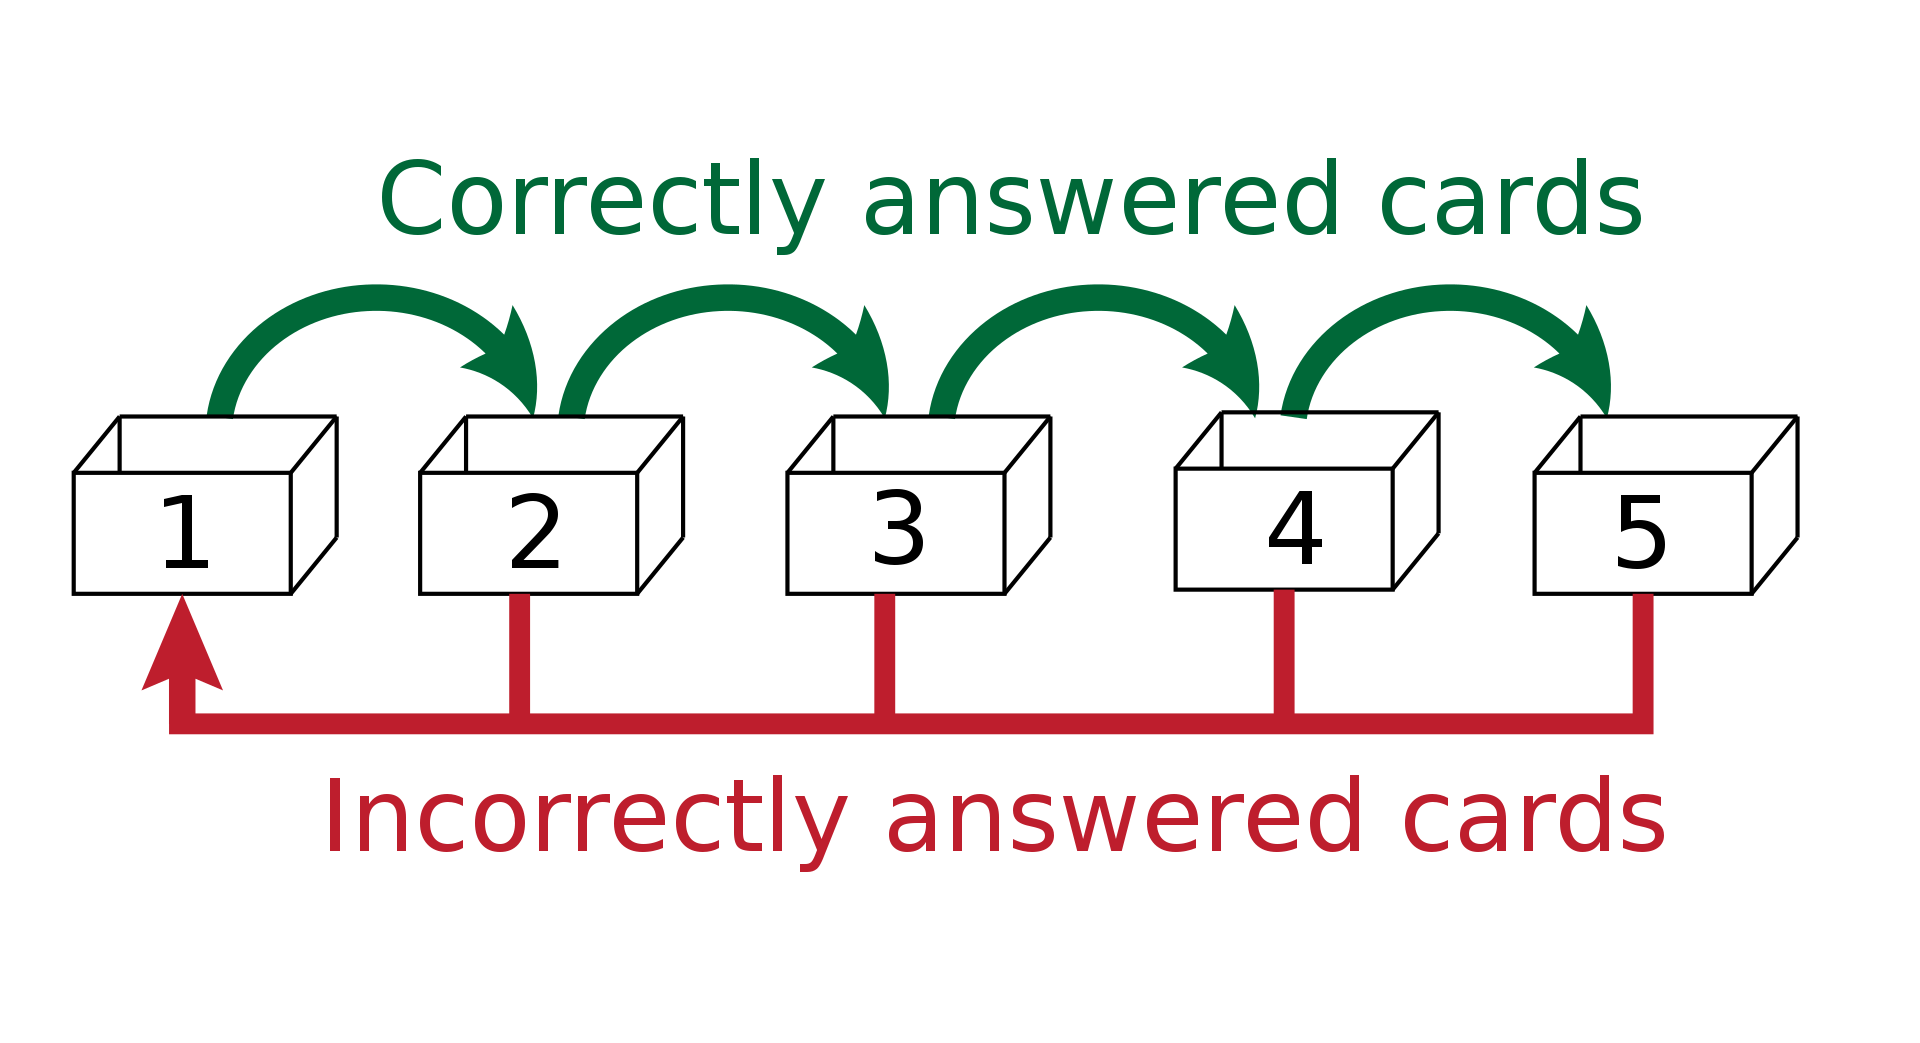
\includegraphics[width=0.5\textwidth]{leitner_system}
\caption{Ilustracja reprezentująca system wykorzystujący fiszki.}
\label{fig:leitner}
\end{figure}
%https://en.wikipedia.org/wiki/Spaced_repetition#/media/File:Leitner_system_alternative.svg

Sposób Leitnera, mimo że skuteczny, jest żmudny do implementacji. Uczeń musi napisać ręcznie wszystkie fiszki, zrobić lub zakupić kilka pudełek o podobnym rozmiarze, rozkładać ten obszerny zestaw za każdym razem, gdy chce powtórzyć materiał. Tym samym traci mobilność, która jest dużą zaletą fiszek. W tym miejscu z pomocą przychodzi nauka języków wspomagana komputerowo (ang. {\english{Computer-Assisted Language Learning}}, CALL). Jest to rozwijana od lat pięćdziesiątych dwudziestego wieku dziedzina wykorzystująca komputery do poprawiania umiejętności językowych \citep{bib:konferencjaCALLhistory}. Ten sposób podejścia do problemu zrzuca z barków uczniów część problemów z tworzeniem fiszek, a wraz z popularyzacją urządzeń takich jak smartfony czy tablety zwraca mobilność nauki. 

Dużą zaletą komputerowo wspomaganej nauki jest możliwość wykorzystania algorytmów do polepszenia jakości zapamiętywania informacji. SM-2 to naśladujący papierowy system Leitnera algorytm autorstwa Piotra Woźniaka stworzony na potrzeby aplikacji SuperMemo\footnote{\url{https://www.supermemo.com/pl}}. W algorytmie SM-2 należy podzielić wiedzę na najmniejsze możliwe części, po czym po każdej powtórce przydzielić wartość od zera do pięciu oznaczającą jakość zapamiętania danej informacji. Na podstawie tej wartości wyliczany jest \textit{współczynnik łatwości} (ang. \english{easiness factor}), a na jego podstawie generowane są pytania w przyszłej sesji powtórek \cite{bib:wozniak}. Sama aplikacja SuperMemo okazała się umiarkowanym sukcesem, jednak algorytm SM-2 cieszy się ogólnym uznaniem i jego zmodyfikowane wersje występują w najpopularniejszych narzędziach komputerowo wspomaganej nauki języków, takich jak Anki\footnote{\url{https://apps.ankiweb.net/}} czy Mnemosyne\footnote{\url{https://mnemosyne-proj.org/}}.

Algorytm powtórek w interwałach (ang. \english{spaced repetition}), którego implementacją jest wyżej wspomniany SM-2, został poddany wielokrotnym badaniom \cite{bib:artykulAlzheimer,bib:artykulSpaced}. Wskazują one nie tylko na poprawę jakości zapamiętywania danego materiału, ale też na ogólną poprawę pamięci, szczególnie u osób chorujących na chorobę Alzheimera lub inne schorzenia związane z pogorszeniem umiejętności zapamiętywania \cite{bib:artykulAlzheimer}. Metoda powtórek w interwałach jest szczególnie użyteczna w nauce słownictwa języków obcych. Jest to spowodowane faktem, że informacje do przyswojenia są liczne, lecz małe. Tę samą zasadę można wykorzystać przy nauce znaków kanji. 

Analiza rozwiązań dostępnych na rynku i badań wskazuje na komercyjny i naukowy sukces metody powtórek w interwałach. To zdroworozsądkowe podejście ma realny wpływ na szybkość i jakość przyswajania wiedzy. Przez ostatnie kilkadziesiąt lat próbowano udoskonalić ten względnie prosty algorytm z użyciem np. metod sztucznej inteligencji do wyliczania interwałów \cite{bib:internetNN, bib:lstms}. Takie podejście ma mieszane rezultaty, nie jest jasne jak realny jest wpływ optymalizacji długości interwału na jakość nauki \cite[rozdział 6]{bib:ksiazkaEssays}.

\section{Rozwiązania dostępne na rynku}

Aktualnie formą nauczania języków wspomaganą komputerowo cieszącą się szerokim zainteresowaniem jest jej poddziedzina, czyli nauczanie języków obcych wspomagane przez urządzenia mobilne (ang. \english{Mobile-Assisted Language Learning, MALL}) \cite{bib:artykulDuolingo}. Największą popularnością \cite{bib:internetDuolingo,bib:artykulDuolingo} cieszy się aplikacja \href{https://pl.duolingo.com/}{Duolingo}\footnote{\url{https://pl.duolingo.com/}}, która umożliwia naukę pokaźniej listy języków (aż czterdziestu trzech na czas pisania tej pracy) z urządzenia mobilnego lub strony internetowej. Jednym z powodów dobrego przyjęcia Duolingo przez uczniów języków obcych jest podejście bogate w gry i zabawy, motywujące użytkownika przez punkty, nagrody i rankingi \cite{bib:artykulDuolingo,bib:duolingoHLR}. Aplikacja nie wymaga od użytkownika dużego zaangażowania. Tworzenie własnych zestawów fiszek nie jest konieczne, wystarczy codziennie wykonać kilkanaście zadań wygenerowanych przez system. 

Innym, bardziej angażującym użytkownika programem chętnie wykorzystywanym do nauki jest \href{https://apps.ankiweb.net/}{Anki}\footnote{\url{https://apps.ankiweb.net/}}. Jest to aplikacja oferująca większą możliwość dostosowania jej do własnych potrzeb, z tego powodu nie jest ograniczona do nauki języków obcych. Użytkownik ma możliwość stworzenie własnego zestawu do nauki złożonego z fiszek, który jest później przyswajany w interwałach zgodnie z zasadą powtórek w interwałach. Zaletą Anki jest opcja eksportowania i dzielenia się zestawami między użytkownikami. 

Wyżej wspomniane programy są często używane przez uczniów języka japońskiego i znaków kanji, jednak nie są wyspecjalizowane pod ich potrzeby. Przykładem aplikacji dostosowanej do amatorów japońskiego alfabetu jest \href{https://www.wanikani.com/}{WaniKani}\footnote{\url{https://www.wanikani.com/}}. Ta aplikacja webowa i mobilna obiecuje uczniom nauczenie się 2000 znaków kanji i 6000 słów w nieco dłużej niż rok. Używa metody powtórek w interwałach w swojej implementacji ustrukturyzowanego kursu, który jest przeznaczony dla początkujących i pozwala rozwinąć się do biegłego posługiwania się kanji. Aplikacja jest gorzej dostosowana do uczniów o zaawansowanym lub średniozaawansowanym poziomie, ponieważ nie da się dopasować jej pod własne potrzeby językowe. 

\section{Nauka języka japońskiego i znaków kanji}

Ważną kwestią przy nauce kanji, zarówno metodami tradycyjnymi jak i z wykorzystaniem komputerowego wspomagania, jest podejście do przyswajanego materiału. Najważniejszą i obowiązkową kwestią jest zapamiętanie wyglądu i pisowni znaku. Aby wspomóc ten proces, można użyć wskazówek mnemonicznych, czyli pewnego skojarzenia między znaczeniem znaku a jego wyglądem.
%obrazek z mnemonika
Kolejną wskazówką do nauki mogą być klucze, czyli elementy znaku dzielące ich zbiór na podkategorie. Ten podział został stworzony na potrzeby słowników i charakteryzuje znaki na podstawie ich najważniejszgo elementu (podznaku). 
%obrazek?

Wraz z opanowaniem pisowni należy zaznajomić się z czytaniem chińskim (jap. \japanese{音読み, onyomi}) i rodzimym japońskim (jap. \japanese{訓読み, kunyomi}). Na nieszczęście uczniów języka japońskiego znaki kanji nie są czytane jednoznacznie i większość z nich ma przynajmniej wyżej wspomniane dwa czytania (wiele z nich ma kilka w ramach \japanese{onyōmi} lub \japanese{kunyōmi}). Na przykład można wziąć znak \japanese{人}, który oznacza człowieka. Jeżeli chcemy powiedzieć poprostu \textit{człowiek}, użyjemy czytania japońskiego -- \japanese{hito}. Jeżeli zechcemy powiedzieć \textit{Japończyk}, użyjemy czytania sinojapońskiego - \japanese{日本\textbf{人}, Nihon\textbf{jin}}. Jak można się zasugerować po powyższym przykładzie, rodzimego czytania często używa się tam, gdzie znak występuje w słowie samodzielnie, a sinojapońskiego tam, gdzie towarzyszą mu inne znaki. Jest to jednak tylko wskazówka, a nie zasada.
 
Aby urozmaicić naukę czytania znaków kanji można połączyć ją z nauką słów, w których ów znak występuje. Takie podejście wzbogaca zasób słownictwa ucznia i ułatwia zapamiętanie czytań danego znaku przez różnorodne przykłady. Kolejnym możliwym sposobem na połączenie nauki znaków z nauką ogólnie rozumianego języka japońskiego jest załączenie ćwiczeń zawierających całe zdania. Umożliwi to użytkownikom o bardziej zaawansowanym poziomie powtarzać różne znaki w jednym ćwiczeniu oraz rozwinie ich ogólne umiejętności językowe. 

Inną kwestią, często lekceważoną przez samouków, jest kolejność stawiania kresek przy pisaniu znaku. Ten sam znak  może  wyglądać zupełnie inaczej, jeżeli nieumiejętnie postawimy kolejne linie, z których się składa. Dlatego istotnym jest, żeby w swoją naukę wkomponować dużo pisania ręcznie, nawet jeśli w naszych czasach jest to coraz mniej popularne. Na wprost użytkownikom wychodzą tutaj też aplikacje, które umożliwiają ćwiczenie pisania przez na przykład rysowanie na ekranie. Uważnie wodząc palec lub długopis po ekranie według instrukcji można wyrobić dobre nawyki, które potem należy utrwalić na kartce.

Podobnie jak inne języki, japoński posiada swój własny system egzaminów przeznaczonych dla obcokrajowców. Egzaminy JLPT (jap. \japanese{日本語能力試験} ang. \english{Japanese Language Proficiency Test}) wydzielają pewne poziomy, które określają umiejętności językowe ucznia. W języku japońskim te poziomy oznacza się literą N oraz cyfrą od 1 do 5, gdzie N5 to najniższy, a N1 najbardziej biegły. Do zdania każdego z tych egzaminów potrzebny jest rosnący z poziomu na poziom zasób kanji. Zaczynając od niewielkich liczb jak około sto dla N5 i trzysta dla N4, kończymy na ponad dwu tysiącach dla pełnej biegłości w pisaniu i czytaniu według egzaminatorów.

Podział znaków kanji według trudności wygląda inaczej dla rodzimych mieszkańców Japonii. Jest on ułożony względem systemu szkolnictwa publicznego, podzielony na klasy w których uczniowie poznają dane znaki. Do zestawu dwu tysięcy znaków wymaganych w szkole, czyli \japanese{常用漢字, jōyō kanji} dochodzi 846 znaków \japanese{人名用, jinmeiyō}, które są dopuszczane w imionach i nazwiskach, mimo że nie należą do \japanese{jōyō kanji}.

Nauka znaków kanji to wieloetapowy proces. Aplikacje i inne pomoce naukowe przeznaczone do tego celu mogą być wysoko wyspecjalizowane, aby jak najbardziej ułatwić przyswajanie informacji.
%%%%%%%%%%%%%%%%%%%%%%%%


% TODO
\chapter{Wymagania i narzędzia}
\label{ch:wymagania-i-narzedzia}

\section{Wymagania funkcjonalne i niefunkcjonalne}

\subsection{Wymagania funkcjonalne}

Wymagania funkcjonalne zostały określone jako lista funkcjonalności z przypisanymi priorytetami, przedstawiona w formie tabeli \ref{id:tab:wymagania}. Najważniejsze są wymagania określone priorytetem Krytyczny, potem Ważny, następnie Niski, najmniejszą wagę mają te z oznacznikiem Opcjonalny. 

\begin{table}[] 
\centering
\caption{Tabela przedstawiająca wymagania funkcjonalne zestawione z priorytetami.}
\label{id:tab:wymagania}
\begin{tabular}{p{0.8\textwidth}|p{0.2\textwidth}}
przypadek użycia & priorytet \\ \hline
Użytkownik może przeglądać listę znaków kanji podzielonych na predefiniowane kategorie  &  Krytyczny   \\
Użytkownik może uczyć się wybranego zestawu znaków według metody powtórek w interwałach, w której najtrudniejsze dla niego znaki będą się pojawiały w najkrótszych interwałach & Krytyczny \\
Użytkownik może zalogować się loginem i hasłem jako uczeń lub nauczyciel & Ważny \\
Użytkownik może się zarejestrować & Ważny \\
Administrator ma dostęp do osobnego panelu administracyjnego, na którym może zarządzać uprawnieniami użytkowników & Ważny \\
Zalogowany użytkownik może tworzyć własne zestawy znaków & Ważny \\
Nauczyciel może tworzyć grupy użytkowników, którzy uczą się razem & Ważny \\
Nauczyciel może zadać zadanie domowe wybranej grupie użytkowników & Ważny \\
Użytkownik może poprosić przy rejestracji o uprawnienia nauczyciela & Niski \\
Nauczyciel może sprawdzać postępy uczniów i komentować ich podejścia & Niski \\
W trakcie nauki uczeń może ćwiczyć pisanie rysując na telefonie & Niski \\
Użytkownik ma dostęp do statystyk danego podejścia & Niski \\
Zalogowany użytkownik może dzielić się swoimi zestawami znaków za pomocą linku & Opcjonalny \\
\end{tabular}
\end{table}

\subsection{Wymagania niefunkcjonalne}
Wymagania niefunkcjonalne, w odróżeniu od funkcjonalnych, nie opisują konkretnych zachowań systemu, a pewne cechy, które określają ogólne zachowanie systemu. Dla aplikacji stworzonej na potrzeby tej pracy wymagania niefunkcjonalne zostały określone w formie listy cech. 
\begin{itemize}
\item Aplikacja ma przechowywaną lokalnie na telefonie użytkownika bazę danych ze znakami kanji, ich złożeniami i przykładowymi zdaniami nieprzekraczającą 20~MB. 
\item Podstawowa funkcjonalność aplikacji jest dostępna offline.
\item System bezpiecznie przechowuje dane użytkowników w bazie danych hostowanej w chmurze.
\item Aplikacja jest skierowana do osób operujących językiem angielskim.
\item Aplikacja jest skierowana do użytkowników urządzeń mobilnych z systemem Android w wersji co najmniej 10.0.
\end{itemize}

\section{Diagramy przypadków użycia}
Ze względu na dość dużą liczbę przypadków użycia, zostały one zaprezentowane jako osobne diagramy UML dla każdego z aktorów. Diagram przypadków użycia dla Ucznia jest przedstawiony na rysunku \ref{fig:uczen}, dla Nauczyciela \ref{fig:nauczyciel}, dla Administratora \ref{fig:admin} a dla Gościa \ref{fig:guest}. Gość to użytkownik niezalogowany. Uczeń do użytkownik zalogowany, a Nauczyciel ma dodatkowo nadane prawa nauczycielskie. Administrator to użytkownik z dostępem do panelu administratora. Nie ma przeszkód, żeby użytkownik był jednocześnie Nauczycielem i Administratorem lub Uczniem i Administratorem.
\begin{figure}[]
\centering
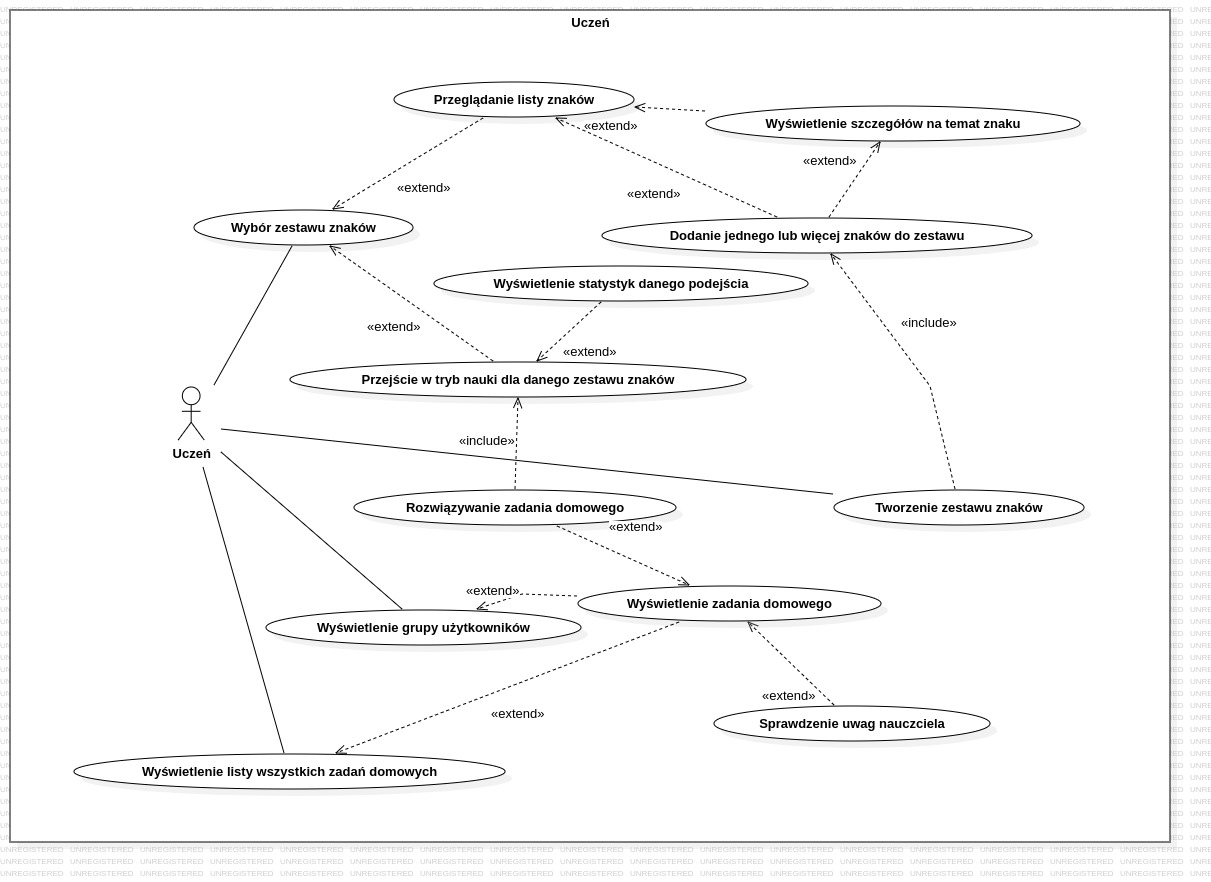
\includegraphics[width=\textwidth]{Uczen}
\caption{Diagram przypadków użycia dla Ucznia.}
\label{fig:uczen}
\end{figure}
\begin{figure}[]
\centering
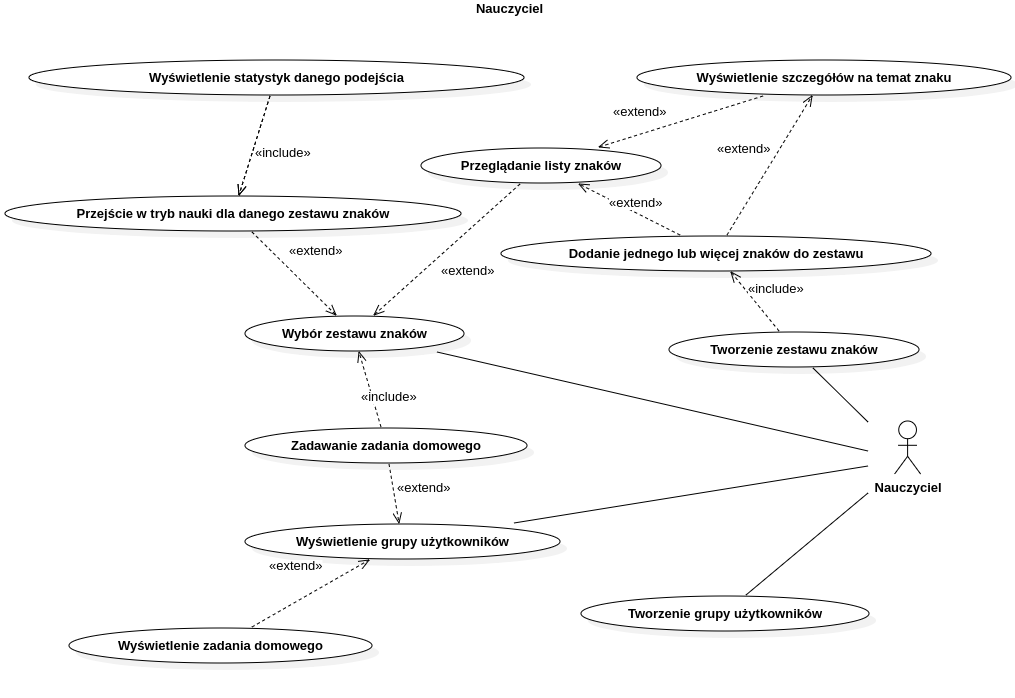
\includegraphics[width=\textwidth]{Nauczyciel}
\caption{Diagram przypadków użycia dla Nauczyciela.}
\label{fig:nauczyciel}
\end{figure}
\begin{figure}[]
\centering
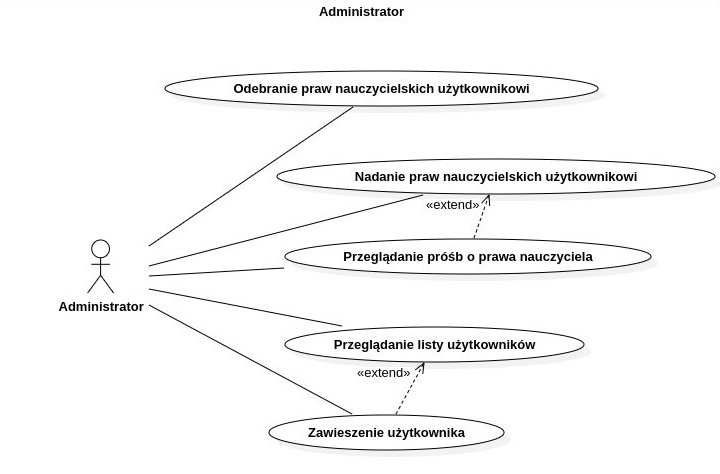
\includegraphics[width=\textwidth]{Admin}
\caption{Diagram przypadków użycia dla Administratora.}
\label{fig:admin}
\end{figure}
\begin{figure}[]
\centering
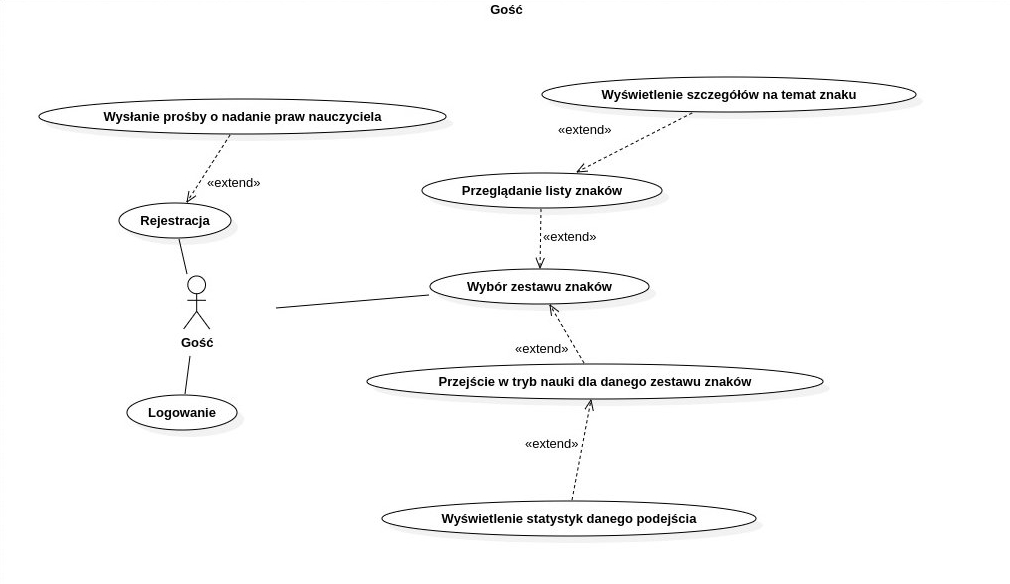
\includegraphics[width=\textwidth]{Gość}
\caption{Diagram przypadków użycia dla Gościa.}
\label{fig:guest}
\end{figure}


%\begin{itemize}
%\item wymagania funkcjonalne i niefunkcjonalne
%\item przypadki użycia (diagramy UML) -- dla prac, w których mają %zastosowanie
%\item opis narzędzi, metod eksperymentalnych, metod modelowania %itp.
%\item metodyka pracy nad projektowaniem i implementacją -- dla %prac, w których ma to zastosowanie
%\end{itemize}

\section{Opis narzędzi}

%
\subsection{Aplikacja mobilna}
%android 10, java, androidstudio, emulator pixel7
%sqlite3
Aplikacja została napisana w języku programowania Java na platformę Android w wersji 10 lub wyższej. Programiści aplikacji przeznaczonych na Androida zwykle wybierają między językami Java i Kotlin (chociaż są interoperacyjne, więc można je łączyć). Kotlin jest językiem stworzonym przez firmę JetBrains, który działa na maszynie wirtualnej Javy. Język ten powstał między innymi aby wyeliminować niektóre problemy Javy, takie jak błędy odwołania (ang. \english{null pointer exceptions}). Kotlin w aplikacjach na Android ma rosnącą popularność. W 2017 został ogłoszony przez firmę Google jako oficjalny język oprogramowania na ten system \cite{bib:internetKotlin17}, a w 2019 jako język preferowany \cite{bib:internetKotlin19}. Według dokumentacji ponad 60 procent profesjonalnych developerów w dziedzinie aplikacji mobilnych na Androida wybiera Kotlin \cite{bib:internetKotlin19}.

Mimo zalet tego nowocześniejszego języka, w aplikacji opisywanej w tej pracy postawiono na Javę. Jest to głównie spowodowane osobistymi pobudkami, takimi jak większa pewność w tym języku i sytuacja na rynku pracy. Dużą zaletą Kotlina i środowiska programistycznego Android Studio jest możliwość konwersji kodu w Javie na kod w Kotlinie. Ta cecha, wraz z interoperacyjnością tych dwóch języków, umożliwia dalszy rozwój aplikacji lub całkowitą migrację na Kotlina w przyszłości. 

%api version 33 - min ver 29 - java 8 support
Przy tworzeniu aplikacji na platformę Android należy wybrać minimalną oraz docelową wersję zestawu narzędzi dla programistów (ang. \english{software development kit}, SDK). W aplikacji opisywanej w tej pracy minimalna wersja to 29 (Android 10), a docelowa 33 (Android 13). Wybór minimalnej wersji zestawu narzędzi jest uzasadniony tym, że 81,9 procent użytkowników tego systemu posiada minimalnie Androida 10 \cite{bib:internetapilevels}. Docelowa wersja jest narzucona przez sklep Google Play. 

Do tworzenia aplikacji użyto środowiska Android Studio Giraffe\footnote{\url{https://developer.android.com/studio/releases/past-releases/as-giraffe-release-notes}}. Android Studio to oficjalnie wspierane środowisko programistyczne dla developerów na platformę Android rozwijane przez firmę JetBrains. Zaprezentowane w 2013 roku, niedługo później zastąpiło wcześniej dominujące Eclipse. Android Studio oferuje bogaty wachlarz udogodnień dla programistów, takich jak:
\begin{itemize}
\item sugestie poprawek kodu dostosowane do Androida,
\item graficzny edytor wyglądu aplikacji z dynamicznym podglądem,
\item wbudowany emulator urządzenia umożliwiający uruchomienie i debugowanie aplikacji.
\end{itemize}
 
\subsection{Lokalna baza danych z informacjami dotyczącymi języka japońskiego}

Do zrealizowania aplikacji opisywanej w tej pracy kluczowym elementem było znalezienie odpowiedniego źródła wiedzy na temat kanji, słów i zdań w języku japońskim. Aby zachować najważniejszą funkcjonalność aplikacji (przeglądanie znaków, uczenie się zestawów) w trybie offline, zdecydowano się na bazę danych przechowywaną lokalnie na urządzeniu każdego z użytkowników. 

Stworzenie tej aplikacji i pracy inżynierskiej jest możliwe dzięki projektowi Kanjium\footnote{\url{https://github.com/mifunetoshiro/kanjium}}. Jest to darmowa baza danych złożona z kilku plików (EDICT, KANJIDIC, KRADFILE) należących do  \english{Electronic Dictionary Research and Development Group} (EDRDG)\footnote{\url{https://www.edrdg.org/edrdg/licence.html}} Informacje na temat partykuł, fonetyki, homonimów, akcentu tonicznego i inne modyfikacje do wyżej wspomnianych plików są autorstwa Urosa Ozvatica. Na potrzeby aplikacji opisywanej w tej pracy baza została okrojona z niepotrzebnych części takich jak dane o synonimach, przysłowiach czy odmiany czasowników, aby jej rozmiar umożliwiał lokalne przechowywanie na urządzeniach użytkowników. Baza danych Kanjium została wykorzystana w tej pracy zgodnie z licencjami grupy EDRDG oraz autora poprawek Urosa Ozvatica.
%https://github.com/mifunetoshiro/kanjium
%https://www.edrdg.org/edrdg/licence.html
%https://creativecommons.org/licenses/by-sa/4.0/

Ponieważ wyżej opisana baza danych zawiera pewne niezmieniające się informacje, jest dostępna dla aplikacji w trybie tylko do odczytu. W przypadku znaczących zmian w standardzie języka japońskiego wymuszających zmiany w bazie, należałoby ją zaktualizować w formie nowej wersji aplikacji.

\subsection{Autoryzacja użytkowników i baza danych}
%firebase auth, firestore
Do zaimplementowania autoryzacji oraz bazy danych zawierającej informacje na temat zalogowanych użytkowników wykorzystano rozwiązanie Firebase\footnote{\url{firebase.google.com/}}. Jest to komplet funkcjonalności oferowanych developerom aplikacji mobilnych, webowych, gier i innych. W aplikacji opisywanej w tej pracy z kompletu narzędzi wykorzystano mechanizm autoryzacji użytkowników i Firestore, czyli bazę danych NoSQL. 

Autoryzacja użytkowników z użyciem Firebase dostarcza programistom łatwe w użyciu metody, które umożliwiają logowanie się użytkowników przez email i hasło lub konto na wybranych portalach społecznościowych. W celu dalszego ułatwienia implementacji Firebase oferuje gotowy interfejs użytkownika przeznaczony do logowania, jednak w tej pracy nie wykorzystano tej możliwości. Autoryzacja użytkownika oferowana przez Firebase została wybrana dla aplikacji opisywanej w tej pracy, ponieważ gotowe, bezpieczne rozwiązanie pozwoliło na poświęcenie cennego czasu na implementację bardziej kluczowych funkcjonalności \cite{bib:ksiazkaFirebase}. Warto zauważyć, że Firebase jest płatne od pewnych progów zużycia zasobów, jednak są one praktycznie nieosiągalne dla aplikacji niedostępnej dla szerokiej publiki.

Firestore, czyli baza danych oferowana jako część zestawu narzędzi Firebase, to baza NoSQL zorientowana na dokumenty. Oznacza to, że dane są przechowywane w dokumentach podobnych do formatu JSON. Różnice między bazami danych SQL i NoSQL leżą w ustrukturyzowaniu przechowywanych danych. SQL było rozwijane w czasach, gdy przechowywanie danych było bardzo drogie. Z tego powodu SQL zwraca dużą uwagę na unikanie duplikacji rekordów. Nowocześniejsze rozwiązania NoSQL mogą zajmować więcej miejsca, jednak są wygodniejsze w użyciu dla programistów. Nie mają stale ustalonych kolumn i nie są relacyjne. Ponieważ istnieje wiele rodzajów baz danych NoSQL, należy uważnie wybrać dystrybucję w zależności od potrzeb. Dla aplikacji rozwijanej na potrzeby tej pracy wybrano bazę danych NoSQL zorientowaną na dokumenty, ponieważ jest to najpopularniejsza alternatywa dla klasycznych, tabularycznych baz danych. Dodatkowym atutem jest łatwość użytku z perspektywy programisty, szczególnie we wczesnych fazach rozwoju aplikacji, gdy często zmienia się pomysł na zapisywanie i wykorzystywanie danych. 

\subsection{Panel administratora}
Panel administratora to aplikacja webowa umożliwiająca administratorowi systemu zarządzanie użytkownikami aplikacji mobilnej. Główną funkcjonalnością panelu administratora jest możliwość rozpatrywania wniosków o uprawnienia nauczyciela. Nauczyciel to użytkownik, który posiada dodatkowe przywileje zakładania grup i zadawania im zadań domowych. Użytkownik może poprosić o takie uprawnienia przy zakładaniu konta w aplikacji mobilnej, a administrator zaakceptować lub odrzucić prośbę. Oprócz tego panel administratora oferuje możliwość przeglądania listy użytkowników wraz z ich uprawnieniami i usuwania ich.

Panel administratora korzysta z tego samego systemu uwierzytelniania użytkowników co aplikacja mobilna. Dodatkowo, przy logowaniu sprawdza, czy użytkownik próbujący się zalogować ma uprawnienia administratora. W przypadku, gdy w bazie nie istnieje użytkownik z uprawnieniami administratora, w panelu pojawia się możliwość założenia konta. Zakłada się, że istnieje tylko jedno konto z uprawnieniami administratora, więc opcja założenia dodatkowych kont nie jest przewidziana. W razie potrzeby administrator może zmienić hasło do swojego konta. Panel korzysta z tej samej instancji bazy danych NoSQL co aplikacja mobilna. Dzięki temu jest w stanie modyfikować dane użytkowników. 

Jako framework ułatwiający budowę aplikacji webowej posłużył Angular\footnote{\url{https://angular.io/}} w wersji 17. Angular to otwartoźródłowa platforma służąca do tworzenia aplikacji webowych używająca języka programowania TypeScript i rozwijana przez Google. Ponieważ funkcjonalności panelu administratora są bardzo proste, wybór Angulara sprowadził się tylko do łatwości użytku związanej z wcześniejszą znajomością tej platformy. Dodatkowym atutem tego frameworku jest też wbudowana obsługa narzędzi Firebase, które są wykorzystywane w aplikacji. Do interfejsu użytkownika wykorzystano bibliotekę Bootstrap\footnote{\url{https://getbootstrap.com/}}, która zawiera pewne zestawy szablonów CSS ułatwiających wykonanie estetycznie spójnej aplikacji.

Aby umożliwić szeroki dostęp do panelu administratora, można upublicznić go na własnym serwerze lub wykorzystując \english{hosting}. Na potrzeby tej pracy przestowano darmowy (z pewnymi ogranicznieniami) serwis z pakietu Firebase. Dzięki wykorzystaniu tej usługi można odwiedzić panel administratora\footnote{\url{https://kanjilearningapp-e002b.web.app/}} z dowolnego urządzenia połączonego  z Internetem.

% TODO
\chapter{Specyfikacja zewnętrzna}
\label{ch:04}
%wymagania sprzętowe i programowe
%sposób instalacji
%sposób aktywacji
%kategorie użytkowników
%sposób obsługi
%administracja systemem
%kwestie bezpieczeństwa
%przykład działania
%scenariusze korzystania z systemu (ilustrowane zrzutami z ekranu lub generowanymi dokumentami)

\section{Wymagania sprzętowe i programowe}
Rozwiązanie opisywane w tej pracy dzieli się na dwie części. Z jednej strony można analizować specyfikację zewnętrzną samej aplikacji mobilnej, z której będą korzystać użytkownicy. Jednak należy też opisać sposób zarządzania całym systemem, w tym panelem administratora. Ten drugi przypadek dotyczy osoby lub organizacji, która zarządzałaby systemem aplikacji mobilnej do nauki kanji.

\subsection{Aplikacja mobilna}

Do instalacji aplikacji mobilnej użytkownik musi koniecznie posiadać urządzenie mobilne lub emulator z systemem Android w wersji conajmniej 10. Do funkcjonalności takich jak zarządzanie grupami lub rozwiązywanie zadania domowego jest potrzebny dostęp do internetu, ale nie jest on konieczny do uruchomienia aplikacji, przeglądania znaków oraz nauki predefiniowanych zestawów. 

\subsection{Baza danych i panel administratora}

Aby móc stworzyć swoją instancję systemu obsługującego dane użytkowników aplikacji mobilnej, konieczne jest urządzenie z dostępem do internetu i skonfigurowany projekt w narzędziu Firebase. Do zbudowania projektu będzie potrzebne następujące oprogramowanie:
\begin{itemize}
\item Android Studio\footnote{\url{https://developer.android.com/studio}},
\item Angular w wersji 17\footnote{\url{https://angular.io/}},
\item Node.js w wersji conajmniej 18.13 wraz z npm\footnote{\url{https://nodejs.org/en}},
\item przeglądarka internetowa (testowano na Firefox w wersji 120)\footnote{\url{https://www.mozilla.org/pl/firefox/new/}}
\end{itemize}

\section{Sposób instalacji i aktywacji}

Podobnie jak wyżej, sposób instalacji i aktywacji oprogramowania będzie różny dla docelowego użytkownika aplikacji mobilnej i dla osoby zarządzającej systemem. 

\subsection{Aplikacja mobilna}
Większość popularnych aplikacji mobilnych w systemie Android można wygodnie i bezpiecznie zainstalować za pomocą Sklepu Play\footnote{\url{https://play.google.com/store/}}. W przypadku aplikacji opisywanej w tej pracy nie jest to możliwe, dlatego należy ręcznie pobrać plik z rozszerzeniem \texttt{apk} i otworzyć go przez menadżer plików w celu instalacji. Jeśli w przyszłości aplikacja mobilna byłaby dalej rozwijana, jest możliwość wykupienia dostępu do Sklepu Play dla deweloperów oraz opublikowania aplikacji do pobrania za darmo lub za pewną opłatą. 

Po instalacji użytkownik może od razu przejść do korzystania z okrojonej wersji aplikacji lub zarejestrować się, aby mieć dostęp do pełnej funkcjonalności. Wersja bez rejestracji jest tożsama wersji bez dostępu do internetu, co oznacza brak możliwości przeglądania grup i zadań domowych oraz tworzenia nowych zestawów.

\subsection{Baza danych i panel administratora}

Po zainicjowaniu projektu w platformie Firebase należy podążać za krokami podanymi w dokumentacji\footnote{\url{https://firebase.google.com/docs/android/setup}}\footnote{\url{https://firebase.google.com/docs/web/setup}}, aby dołączyć swój projekt Firebase do aplikacji mobilnej oraz panelu administratora. Istotne jest, aby był to ten sam projekt, dzięki temu możliwa będzie wymiana danych. Po zbudowaniu i wdrożeniu panelu administratora należy założyć konto umożliwiające administrację systemu. 

Przy budowaniu w panelu administratora w trybie produkcyjnym należy zwrócić uwagę na konfigurację, ponieważ rozwiązania Firebase i Angular wydają się nie być w stu procentach kompatybilne. Aby doprowadzić aplikację do działania należy uruchomić komendę budowania z wyłączoną optymalizacją (\texttt{ng build --optimization=false}).

%hosting

\section{Kategorie użytkowników}

Użytkownicy w rozwiązaniu opisywanym w tej pracy dzielą się na cztery rodzaje. 
\begin{itemize}
\item Gość -- użytkownik niezalogowany,
\item Uczeń -- użytkownik zalogowany,
\item Nauczyciel -- użytkownik zalogowany z dodatkowymi uprawnieniami. Może tworzyć grupy i zadawać zadania domowe,
\item Administrator -- użytkownik, który ma dostęp do panelu administratora.
\end{itemize}
Rola administratora może występować równocześnie z rolą ucznia lub nauczyciela, ale Nauczyciel nie może być jednocześnie Uczniem.

%\section{Sposób obsługi} duplikat ze scenariuszami?

\section{Administracja systemu}

Administracja systemu odbywa się za pomocą panelu administratora. Jest to aplikacja webowa połączona z bazą danych w Firebase, która umożliwia użytkownikowi  administratorowi na zarządzanie użytkownikami. Administrator może przeglądać listę użytkowników, usuwać użytkowników, rozpatrzać prośby o uprawnienia nauczyciela. 

Panel administratora zawiera większość funkcjonalności potrzebnych do administracji systemu, jednak w razie potrzeby można skorzystać z obszerniejszych narzędzi dostarczanych przez Firebase. Przykładem może być tymczasowe zawieszenie użytkownika, dodanie nowej formy logowania lub włączenie dwuetapowej weryfikacji.

\section{Bezpieczeństwo}

System pobiera pewne wrażliwe dane na temat użytkowników, takie jak adres mailowy, dlatego ważne są kwestie bezpieczeństwa aplikacji. Narzędzia Firebase wykorzystywane w tej pracy, czyli autoryzacja użytkowników oraz baza danych, posiadają certyfikaty prywatności i bezpieczeństwa ISO 27001, ISO 27017, ISO 27018 oraz SOC 1, SOC 2, i SOC 3\footnote{\url{https://firebase.google.com/support/privacy}}. 
Baza danych jest zabezpieczona regułami (rys. \ref{fig:rules}), które blokują dostęp do danych użytkownikom niezalogowanym, co stanowi kolejną barierę.

\begin{figure}[]
\centering
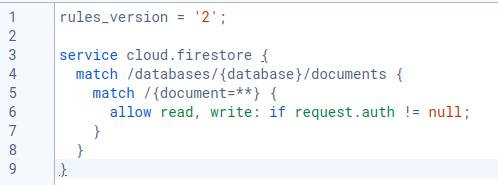
\includegraphics[width=0.5\textwidth]{Firestore}
\caption{Przykład reguł definiujących dostęp do bazy danych.}
\label{fig:rules}
\end{figure}

%\section{Przykład działania} duplikat?
\section{Scenariusze korzystania z systemu}

Scenariusze korzystania z systemu to przykładowe drogi, jakie użytkownik może przejść po systemie opisywanym w tej pracy. Zostaną przedstawione osobno dla aplikacji mobilnej i dla panelu administratora.

\subsection{Aplikacja mobilna}

Scenariusze korzystania z aplikacji mobilnej są przedstawione na rysunku \ref{fig:navgraph}. Przedstawiony na nim diagram pokazuje ścieżki, jakie może podjąć użytkownik rozpoczynając od ekranu startowego (ekran startMenu), paska menu (rys. \ref{fig:menu}) naciskając ikonę plusa (ekran createNewSet) lub ikonę reprezentującą grupę (ekran groupManagement). 

\begin{figure}[]
\centering

\includegraphics[width=0.5\textwidth]{menu}
\caption{Pasek menu znajdujący się w górnej części interfejsu użytkownika aplikacji.}
\label{fig:menu}
\end{figure}

\begin{figure}[]
\centering
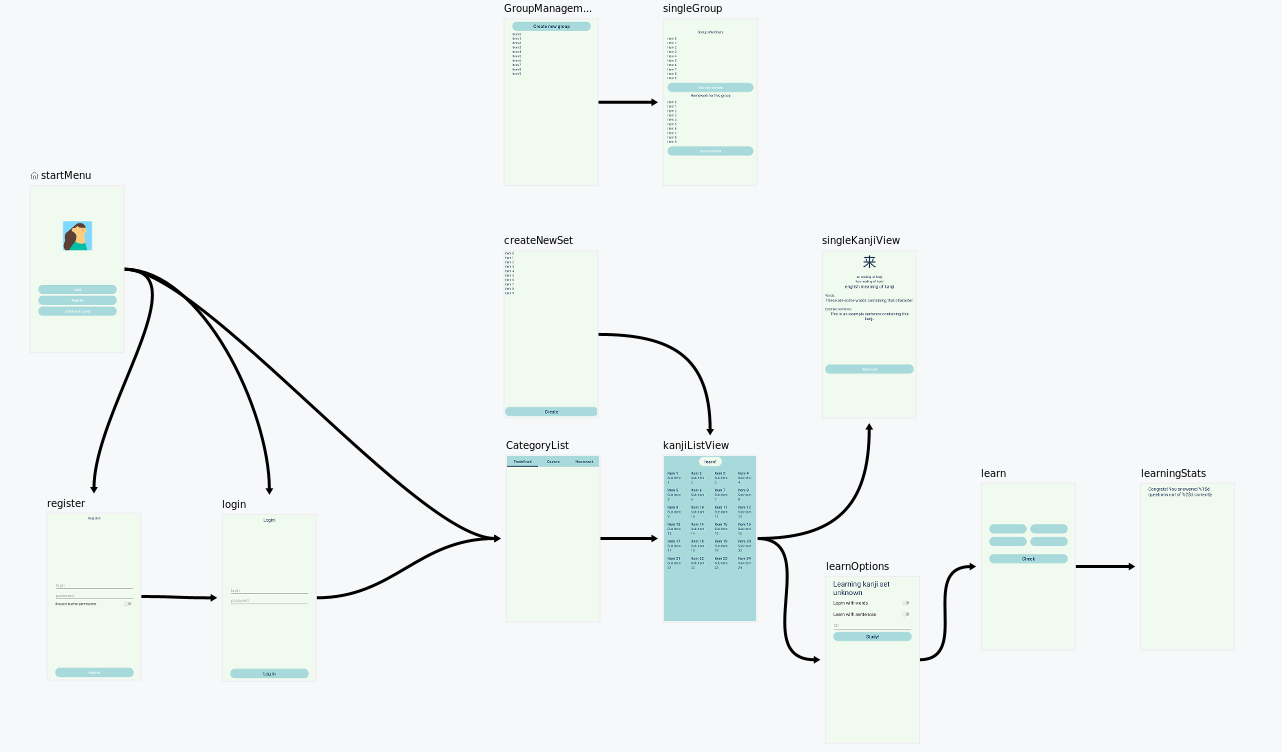
\includegraphics[width=\textwidth]{Navgraph}
\caption{Diagram reprezentujący scenariusze korzystania z systemu.}
\label{fig:navgraph}
\end{figure}

Szczególnym, najbardziej rozwiniętym przypadkiem scenariusza korzystania z aplikacji mobilnej jest sama nauka zestawów (ekran learn). Ponieważ diagram nie pokazuje szczegółów, ten fragment zostanie przedstawiony za pomocą zrzutów ekranu (rys. \ref{fig:study}). 

Użytkownik rozpoczyna od wyboru zestawu z listy (ekran CategoryList na rysunku \ref{fig:navgraph}). Po wybraniu zestawu może obejrzeć znaki, które się w nim znajdują (rys. \ref{fig:list}). Po naciśnięciu przycisku \textit{learn}, użytkownik przechodzi do wyboru opcji podejścia (rys. \ref{fig:options}). Może wybrać liczbę tur oraz w pewien sposób zmodyfikować pytania, które wygeneruje program.  Po przejściu do nauki widoczne jest pytanie, znak którego dotyczy, pole do wprowadzenia odpowiedzi oraz przycisk zatwierdzający (rys. \ref{fig:start}). W kolejnych pytaniach pojawia się dodatkowo informacja o poprawnej odpowiedzi w poprzednim pytaniu (rys. \ref{fig:correct}) lub o niepoprawnej wraz z przykładami, jak należało odpowiedzieć na to pytanie (rys. \ref{fig:incorrect}). Po zakończonym podejściu użytkownik może zobaczyć statystyki (rys. \ref{fig:stats}).


%%%%%%%%%%%%%%%%%%%%%
% WIELE RYSUNKÓW 

\begin{figure}
\centering
\begin{subfigure}{0.3\textwidth}
    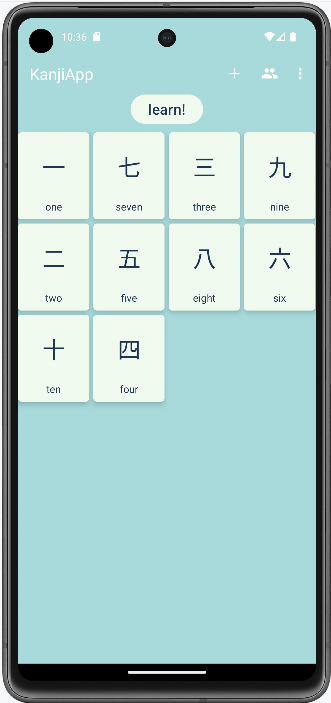
\includegraphics[width=\textwidth]{learn/list}
    \caption{Widok zestawu wybranego do nauki.}
    \label{fig:list}
\end{subfigure}
\hfill
\begin{subfigure}{0.3\textwidth}
   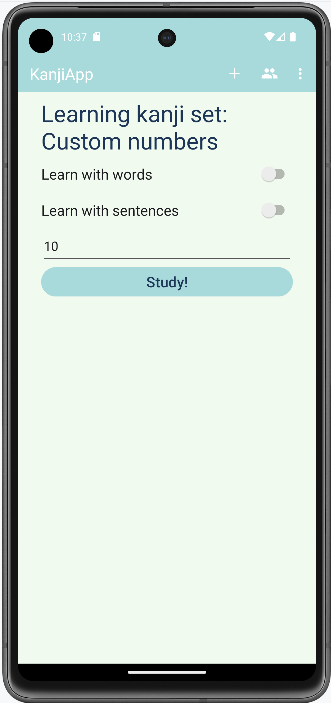
\includegraphics[width=\textwidth]{learn/options}
   \caption{Widok wyboru opcji sesji powtórek.}
   \label{fig:options}
\end{subfigure}
\hfill
\begin{subfigure}{0.3\textwidth}
   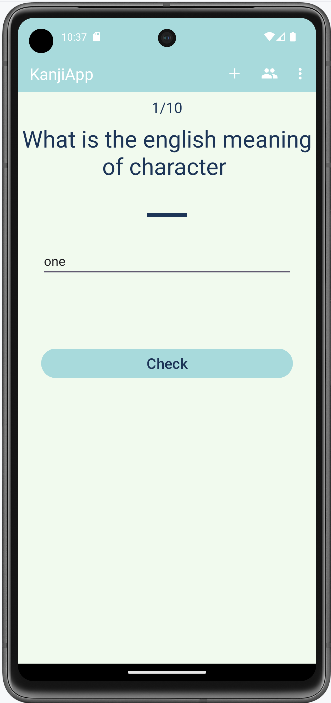
\includegraphics[width=\textwidth]{learn/start}
   \caption{Pierwsze pytanie z wybranego zestawu.}
   \label{fig:start}
\end{subfigure}

 
\begin{subfigure}{0.3\textwidth}
   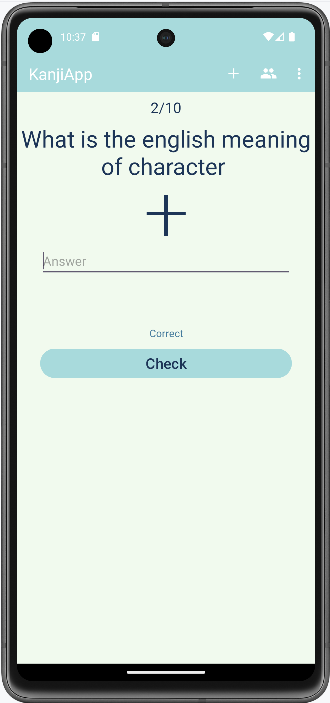
\includegraphics[width=\textwidth]{learn/correct}
   \caption{Kolejne pytanie z informacją o poprawnej odpowiedzi do poprzedniego.}
   \label{fig:correct}
\end{subfigure}
\hfill 
\begin{subfigure}{0.3\textwidth}
   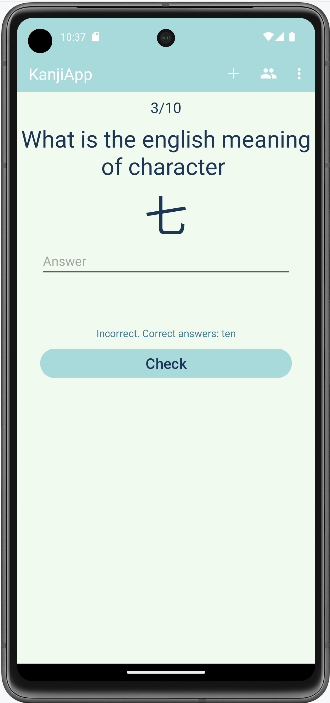
\includegraphics[width=\textwidth]{learn/incorrect}
   \caption{Kolejne pytanie z informacją o niepoprawnej odpowiedzi do poprzedniego.}
   \label{fig:incorrect}
\end{subfigure}
\hfill
\begin{subfigure}{0.3\textwidth}
   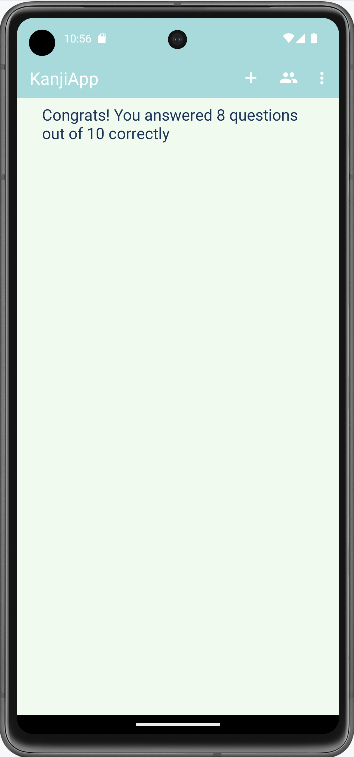
\includegraphics[width=\textwidth]{learn/stats}
   \caption{Ekran ze statystykami podejścia pojawiający się po zakończeniu nauki.}
   \label{fig:stats}
\end{subfigure}
 

\caption{Scenariusz reprezentujący naukę wybranego zestawu.}
\label{fig:study}
\end{figure}
%%%%%%%%%%%%%%%%%%%%%

\subsection{Baza danych i panel administratora}

Aby skorzystać z funkcjonalności panelu administratora, należy się zalogować. Ekran logowania jest przedstawiony na rysunku \ref{fig:login}. Dostęp do panelu mają jedynie użytkownicy o uprawnieniach administratora. Jeżeli konta z takimi uprawnieniami nie ma jeszcze w systemie, użytkownik zostanie o tym powiadomiony (rysunek \ref{fig:alert}) oraz przeniesiony do podstrony umożliwiającej założenie konta (rysunek \ref{fig:register}). Po udanym zalogowaniu lub rejestracji administrator ma dostęp do funkcjonalności panelu, takich jak wyświetlanie użytkowników wraz z ich uprawnieniami oraz możliwością ich usunięcia (rysunek \ref{fig:dashboard}) lub widok próśb o uprawnienia nauczyciela, które może zaakceptować lub odrzucić. Zalogowany administrator ma też możliwość zmiany hasła, co jest przedstawione na rysunku \ref{fig:changepwd}. Nie ma potrzeby wpisywania starego hasła, ponieważ autoryzacja użytkowników Firebase automatycznie sprawdza, czy użytkownik niedawno się logował. Jeżeli od logowania minęło zbyt dużo czasu, użytkownik może ponownie się zalogować i zmienić hasło. 

\begin{figure}[]
\centering
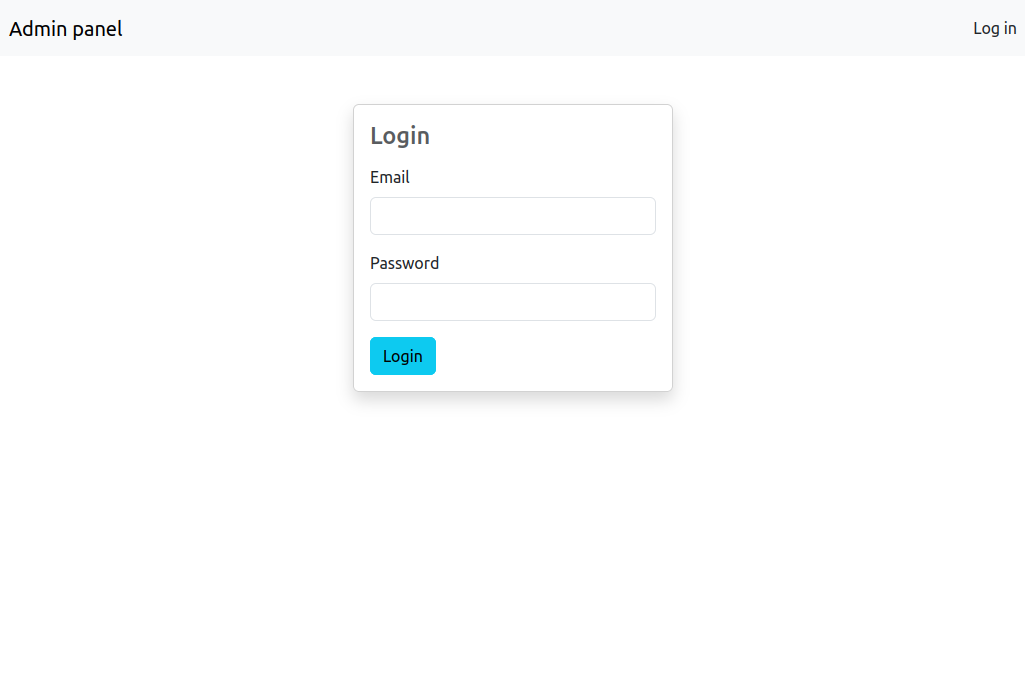
\includegraphics[width=\textwidth]{adminpanel/login}
\caption{Okno logowania.}
\label{fig:login}
\end{figure}

\begin{figure}[]
\centering
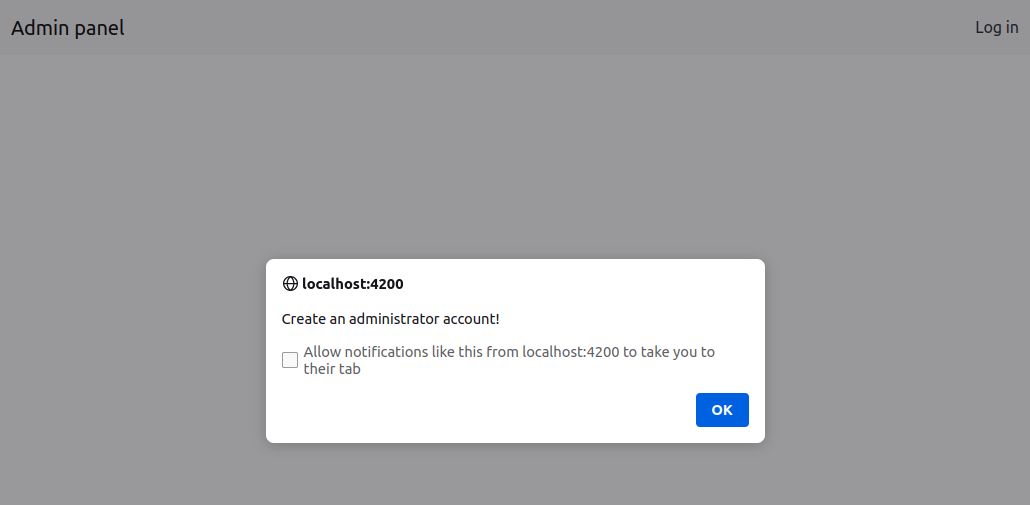
\includegraphics[width=\textwidth]{adminpanel/alert}
\caption{Powiadomienie wyświetlane w przypadku, gdy w bazie nie ma użytkownika z uprawnieniami administratora.}
\label{fig:alert}
\end{figure}

\begin{figure}[]
\centering
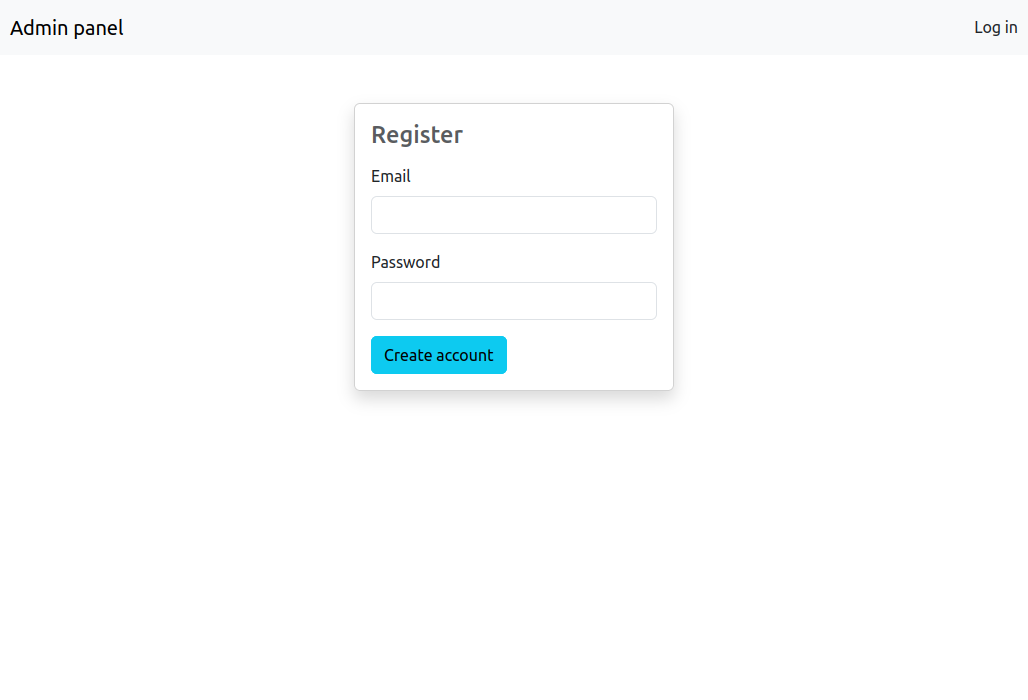
\includegraphics[width=\textwidth]{adminpanel/register}
\caption{Okno rejestracji.}
\label{fig:register}
\end{figure}

\begin{figure}[]
\centering
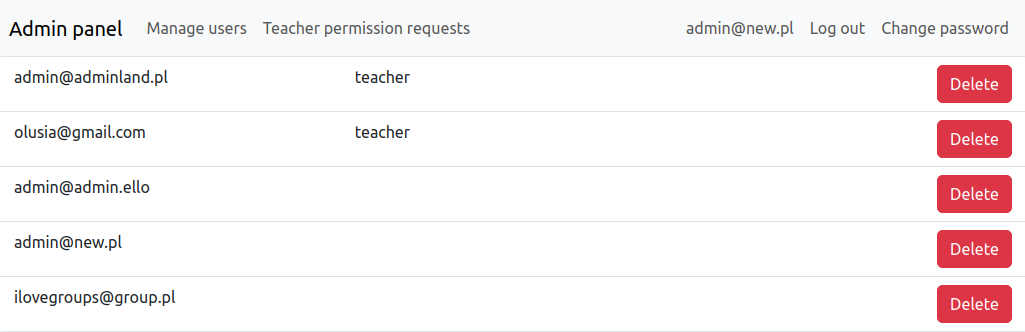
\includegraphics[width=\textwidth]{adminpanel/dashboard}
\caption{Widok wszystkich użytkowników.}
\label{fig:dashboard}
\end{figure}

\begin{figure}[]
\centering
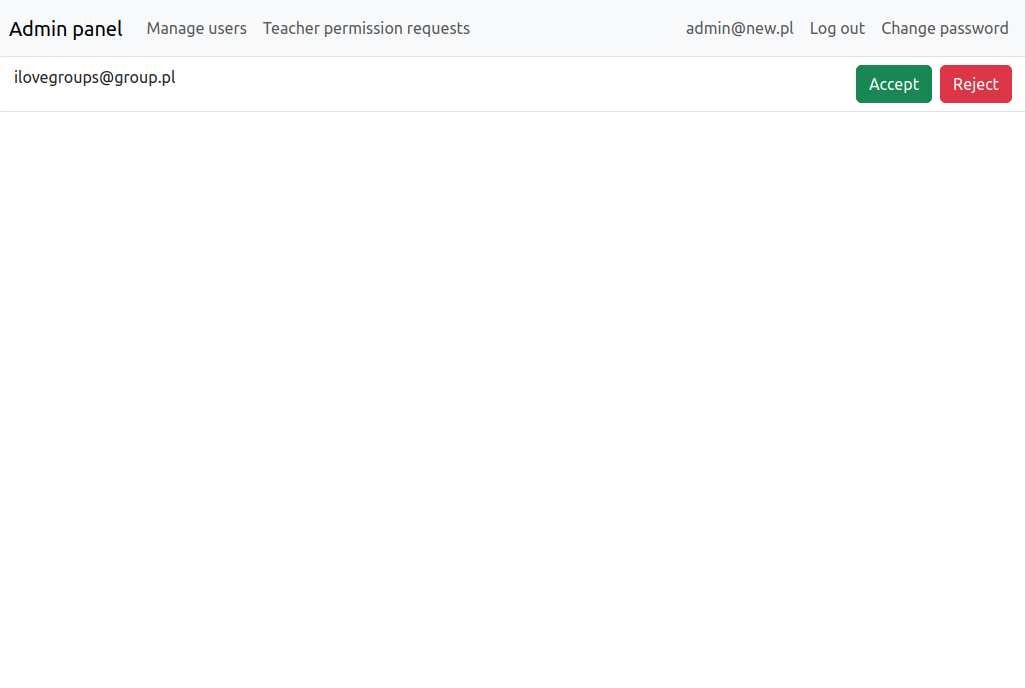
\includegraphics[width=\textwidth]{adminpanel/requests}
\caption{Widok próśb o uprawnienia nauczyciela.}
\label{fig:requests}
\end{figure}

\begin{figure}[]
\centering
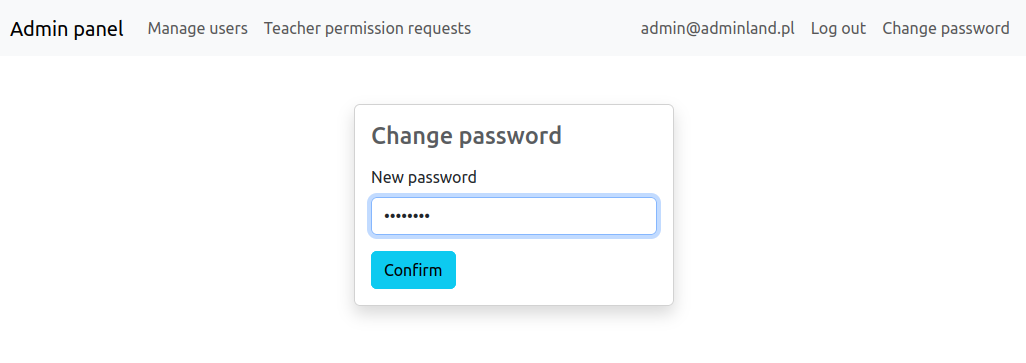
\includegraphics[width=\textwidth]{adminpanel/changepwd}
\caption{Okno zmiany hasła.}
\label{fig:changepwd}
\end{figure}

% TODO
\chapter{Specyfikacja wewnętrzna}
\label{ch:05}

%przedstawienie idei
%architektura systemu
%opis struktur danych (i organizacji baz danych)
%komponenty, moduły, biblioteki, przegląd ważniejszych klas (jeśli występują)
%przegląd ważniejszych algorytmów (jeśli występują)
%szczegóły implementacji wybranych fragmentów, zastosowane wzorce projektowe
%diagramy UML

\section{Architektura systemu}

Architektura systemu została zaprezentowana za pomocą diagramu na rysunku \ref{fig:archi}. Rozwiązanie opisywane w tej pracy składa się z następujących części:
\begin{itemize}
\item aplikacja mobilna do nauki kanji (roz. \ref{sec:1}),
\item lokalna baza danych z danymi dotyczącymi języka japońskiego (roz. \ref{sec:2}),
\item baza danych przechowująca dane użytkowników, ich postępy oraz grupy, do których należą (roz. \ref{sec:3}),
\item panel administratora pozwalający na zarządzanie użytkownikami (roz. \ref{sec:4}),
\end{itemize}

\begin{figure}[]
\centering
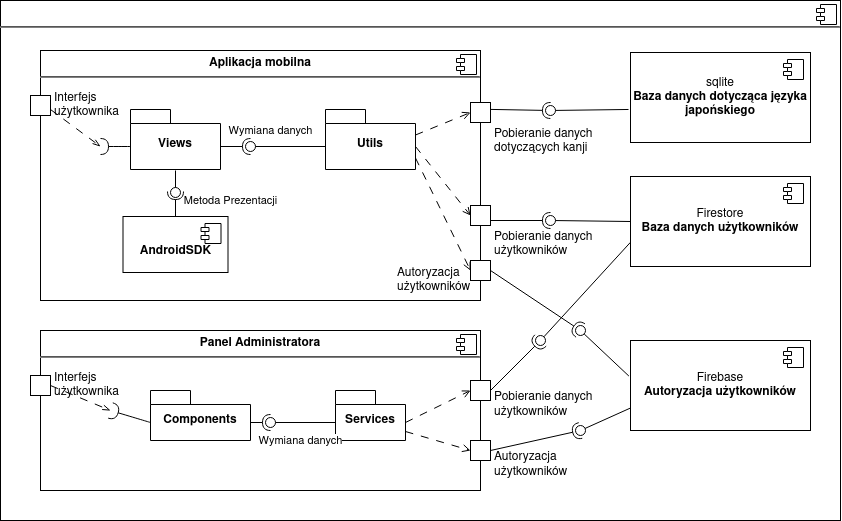
\includegraphics[width=\textwidth]{component}
\caption{Diagram przedstawiający architekturę systemu.}
\label{fig:archi}
\end{figure}

\subsection{Aplikacja mobilna}
\label{sec:1}
%\ksremark{Jakiś diagram modelu / diagram komponentów.}

Większość aplikacji na system operacyjny Android jest napisanych zgodnie z architekturą MVC (\english{Model View Controller}), MVP (\english{Model View Presenter}) lub MVVM (\english{Model View ViewModel}). Wzorzec należy dobrać odpowiednio do rodzaju programu, jednak często wybór sprowadza się do preferencji programistów. 

Według niektórych źródeł wzorzec MVC jest wymuszany przez samą strukturę aplikacji androidowych \cite{bib:internetMVC}. W tej wersji modelem są klasy reprezentujące dane, kontrolerem aktywności lub fragmenty stanowiące logikę działania aplikacji, a widokiem pliki z rozszerzeniem \texttt{xml} reprezentujące wygląd danego okna. Takie podejście nie oddaje do końca prawdy. Widok to statyczny plik \texttt{xml} -- nie jest w stanie sam odświeżać danych. Z tego powodu klasa aktywności oprócz odpowiedzialności kontrolera wykonuje rownież zadania widoku. Konsekwencją tego jest w pewnym sensie zatracenie się sensu architektury MVC, której głównym zadaniem jest rozdzielenie odpowiedzialności modelu, widoku i kontrolera. W większych projektach jest to dużym problemem, ponieważ utrudnia testy jednostkowe aplikacji.

Odpowiedzią na ten problem jest architektura MVP, która w sposób dostosowany do aplikacji Androidowych rozdziela model, widok i odpowiednik kontrolera -- prezenter. Prezenter w tej wersji to osobna klasa w pełni oddzielona od widoku, co umożliwia testowanie jednostkowe logiki aplikacji \cite{bib:lou2016comparison}. We wzorcu MVP jedynie widok dziedziczy po klasach typowych dla Androida, takich jak \english{Activity} lub \english{Fragment}. Wadą architektury MVP jest większa ilość szablonowego kodu, który należy napisać na potrzeby komunikacji między modelem, widokiem i prezenterem. Może to skutkować również mniejszą czytelnością.

Na etapie planowania architektury aplikacji mobilnej wybrano wzorzec MVC. Ponieważ MVC jest powszechny w materiałach edukacyjnych oraz w pewnym sensie wymuszany przez samo środowisko pracy w Androidzie, to podejście pozwoliło na skupienie się na odpowiednim działaniu aplikacji bez większego problemu z projektowaniem architektury systemu. W przypadku dalszego rozwijania aplikacji, również w kwestii testów jednostkowych, warto wykonać refraktoryzację kodu na wzorzec MVP. 

\subsection{Panel administratora}
\label{sec:2}

Panel administratora to aplikacja webowa stworzona w całości dzięki frameworkowi Angular\footnote{\url{https://angular.io/}}. Ponieważ ta aplikacja nie jest zbyt rozbudowana, jej architektura nie jest skomplikowana i nie wymaga modyfikacji narzędzi dostarczanych przez Angular. Częściami aplikacji wykonanej w tym frameworku są komponenty, czyli widoki. Przykładem komponentu jest pasek nawigacyjny, który widnieje w górnej części strony lub część strony odpowiedzialna za logowanie (rys. \ref{fig:login}). Komponent ma plik z rozszerzeniem \texttt{html}, który definiuje wygląd elementu aplikacji oraz klasę w języku Typescript, która odpowiada za logikę. Komponenty używają serwisów, czyli klas wyspecjalizowanych do zarządzania danymi. Angular silnie polega na mechanizmie wstrzykiwania zależności, którego używa do łączenia serwisów z komponentami. 

\section{Organizacja baz danych}

W rozwiązaniu opisywanym w tej pracy występują dwie bazy danych. Pierwsza z nich jest przechowywana lokalnie i dotyczy reguł języka japońskiego, a druga znajduje się na zdalnym serwerze i zawiera dane dotyczące użytkowników i grup.

\subsection{Baza danych dotycząca języka japońskiego}
\label{sec:3}

Dane dotyczące znaków, słownictwa, przykładowych zdań i innych informacji są przechowywane lokalnie w pliku sqlite. Jest on okrojoną wersją bazy danych Kanjium\footnote{\url{https://github.com/mifunetoshiro/kanjium}}, która łączy wiele źródeł informacji na temat języka japońskiego w spójną bazę danych. 

Dzięki projektowi Kanjium powstało bardzo bogate źródło wiedzy na temat języka japońskiego, jednak do zrealizowania aplikacji omawianej w tej pracy nie jest konieczny cały zbiór. Dodatkowo, ponieważ ta baza danych jest przeznaczona do przechowywana lokalnie na urządzeniu każdego z użytkowników, istotny jest mały rozmiar samego pliku. Z tych powodów zdecydowano się na usunięcie pewnych tabel i pozostawienie tylko niezbędnych informacji (rys. \ref{fig:kanjidb}), takich jak słownik kanji (tabela \texttt{kanjidict}), tabele zawierające złożenia znaków (\texttt{edict}, \texttt{compverbs}, \texttt{jukugo}), tabelę \texttt{sentences}, która ma w sobie przykładowe zdania oraz tabelę \texttt{search}, która umożliwia wyszukiwanie znaków przez użytkownika. Pozbyto się danych, które nie są konieczne do zrealizowania nauki znaków kanji, takich jak odmiana czasowników lub przysłowia.

Ostatecznie okrojona baza danych ma rozmiar 18 MB, co nieco przekracza wstępne założenia o bazie nieprzekraczającej 15 MB, jednak przy obecnych rozmiarach pamięci w urządzeniach mobilnych nie powinno to zniechęcić użytkowników od korzystania z aplikacji. W~przyszłości jest możliwość dalszego zmniejszania bazy na przykład przez usuwanie zbędnych wierszy, nie tylko tabel i kolumn.

Diagram przedstawiający schemat bazy danych (rys. \ref{fig:kanjidb}) został wygenerowany przez otwartoźródłowe oprogramowanie schemacrawler\footnote{\url{https://www.schemacrawler.com/}}.
\begin{figure}[]
\centering
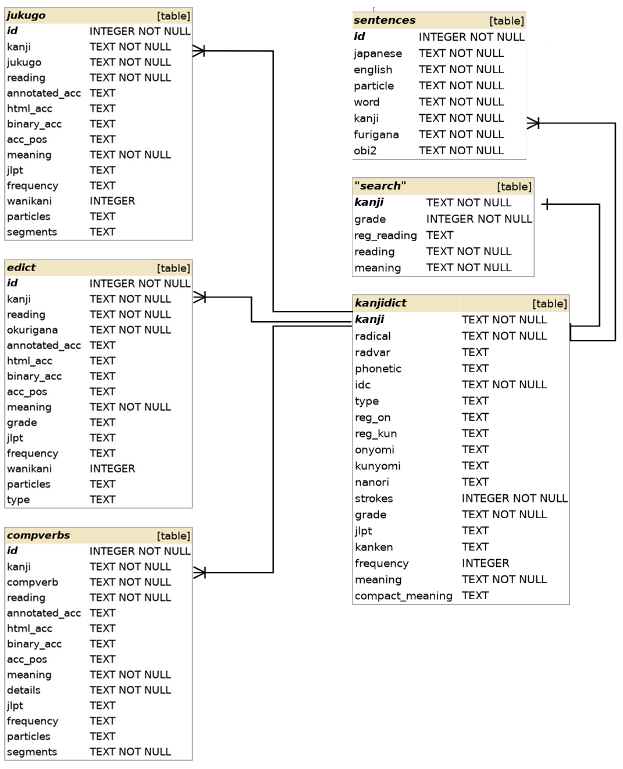
\includegraphics[width=0.8\textwidth]{kanjidbrelations}
\caption{Diagram przedstawiający schemat bazy danych sqlite dotyczących języka japońskiego.}
\label{fig:kanjidb}
\end{figure}

\subsection{Baza danych przechowująca dane użytkowników}
\label{sec:4}

Dane dotyczące użytkowników są przechowywane w bazie danych NoSQL zorientowanej na dokumenty. Na rysunku \ref{fig:firestore} przedstawiono kolekcje jako foldery, które przechowują dokumenty. Dokumenty mogą mieć zagnieżdżone kolekcje, które na diagramie są zaznaczone pogrubionym tekstem. 

\begin{itemize}
\item \texttt{User}: dokument reprezentujący użytkownika, posiada informacje o jego danych i uprawnieniach. Posiada zagnieżdżone kolekcje \texttt{Sets} i \texttt{Predefined} które zawierają dokumenty reprezentujące zestawy do nauki.
\item \texttt{Group}: ten rodzaj dokumentu reprezentuje grupę. Zawiera identyfikatory członków oraz zagnieżdżoną kolekcję zestawów, które do niej należą.
\item \texttt{Set}: dokumenty \texttt{Set} przedstawiają zestaw znaków. W tej bazie danych można przechowywać mapę, co okazało się bardzo pomocne przy zapisywaniu wartości jakości zapamiętywania dla każdego znaku.
\item \texttt{Predefined}: dokumenty \texttt{Predefined} mają strukturę identyczną do dokumentów \texttt{Set}, ale dotyczą zestawów do nauki już zapisanych w kodzie aplikacji.
\end{itemize}

\begin{figure}[]
\centering
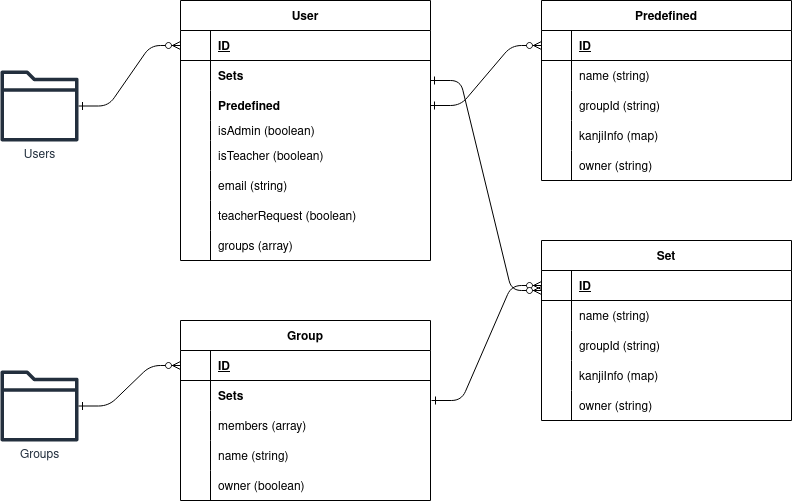
\includegraphics[width=0.8\textwidth]{firestore.drawio}
\caption{Diagram przedstawiający schemat bazy danych zorientowanej na dokumenty.}
\label{fig:firestore}
\end{figure}

\section{Pakiety i klasy}

W tym podrozdziale zostanie opisana struktura projektów aplikacji mobilnej i panelu administratora oraz ważniejsze klasy w tych programach.

\subsection{Aplikacja mobilna}

Kod aplikacji mobilnej został podzielony na pięć pakietów, które odpowiadają za różne części funkcjonowania programu. Pakiety i zależności między nimi zostały zaprezentowane na rysunku \ref{fig:package}. Oprócz nich w repozytorium znajduje się plik \texttt{MainActivity.java}, który pełni rolę punktu startowego programu, zarządzania nawigacją oraz paskiem menu. 

Aplikacja jest zbudowana z następujących pakietów:
\begin{itemize}
\item \texttt{adapters} -- klasy pośredniczące między elementami interfejsu użytkownika i danymi,
\item \texttt{models} -- klasy reprezentujące dane,
\item \texttt{types} -- typy wyliczeniowe,
\item \texttt{utils} -- klasy pomocnicze, służące do komunikacji z bazą danych lub generowania pytań,
\item \texttt{views} -- klasy obsługujące interfejs użytkownika.
\end{itemize} 
\begin{figure}[]
\centering
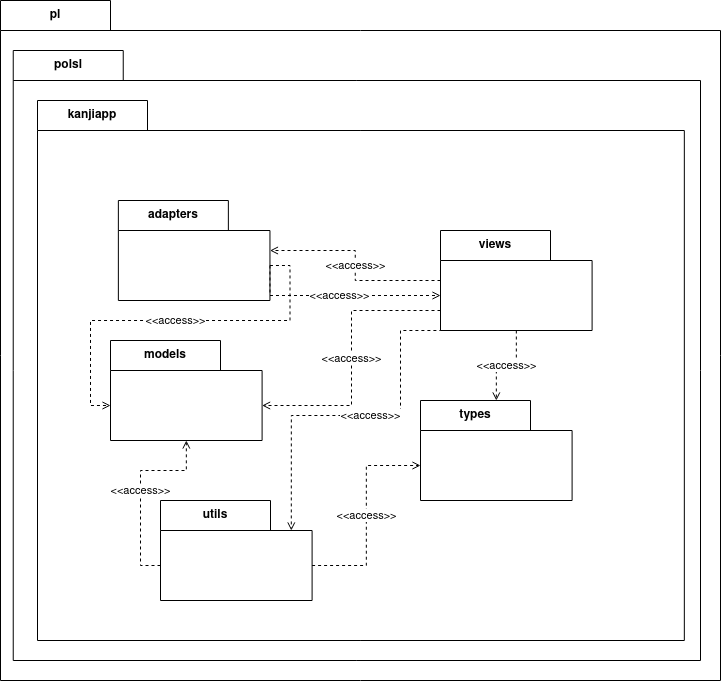
\includegraphics[width=\textwidth]{packages}
\caption{Diagram pakietów aplikacji mobilnej.}
\label{fig:package}
\end{figure}

\subsection{Panel administratora}

Kod panelu administratora składa się z komponentów odpowiedzialnych za interfejs użytkownika, serwisów zarządzających danymi oraz modeli reprezentujących dane. Drzewo na rysunku \ref{fig:dirtree} przedstawia strukturę plików aplikacji, a architekturę na rysunku \ref{fig:archi}.

\begin{figure}
\dirtree{%
.1 src/app/.
.2 component/.
.3 change-pwd.
.3 dashboard.
.3 login.
.3 navbar.
.3 register.
.3 teachers.
.2 models/.
.3 account.
.2 shared/.
.3 auth.service.
.3 data.service.
}
\caption{Struktura plików w kodzie panelu administratora.}
\label{fig:dirtree}
\end{figure}

% TODO
\chapter{Weryfikacja i walidacja}
\label{ch:06}

\section{Sposób testowania w ramach pracy}

Testowanie to proces towarzyszący tworzeniu aplikacji i ściśle z nim powiązany. Aplikacja opisywana w tej pracy została przetestowana w pewnym zakresie, jednak przed wypuszczeniem jej na rynek należałoby go znacznie rozszerzyć.

\subsection{Testy manualne}

Testy manualne były wykonywane przez cały czas rozwoju aplikacji mobilnej oraz panelu administratora. Polegały one na przejściu przez pewną ścieżkę programu w celu wykrycia błędu lub potwierdzenia prawidłowego działania. Najczęściej testy manualne były wykonywane po implementacji pewnej fukcjonalności. Po zakończeniu prac nad rozwojem kodu programy zostały kompleksowo przetestowane. 

Testowanie manualne aplikacji mobilnej było możliwe dzięki emulatorowi urządzenia mobilnego z systemem Android. Użycie emulatora zaoszczędziło dużą ilość czasu oraz nakładu pracy, ponieważ pozwoliło na testowanie bezpośrednio w środowisku developerskim Android Studio. Emulator wykorzystany do testowania w rozwiązaniu opisywanym w tej pracy to Pixel 7 z systemem Android w wersji 13.0 i obsługą sklepu Google Play.

\begin{figure}[]
\centering
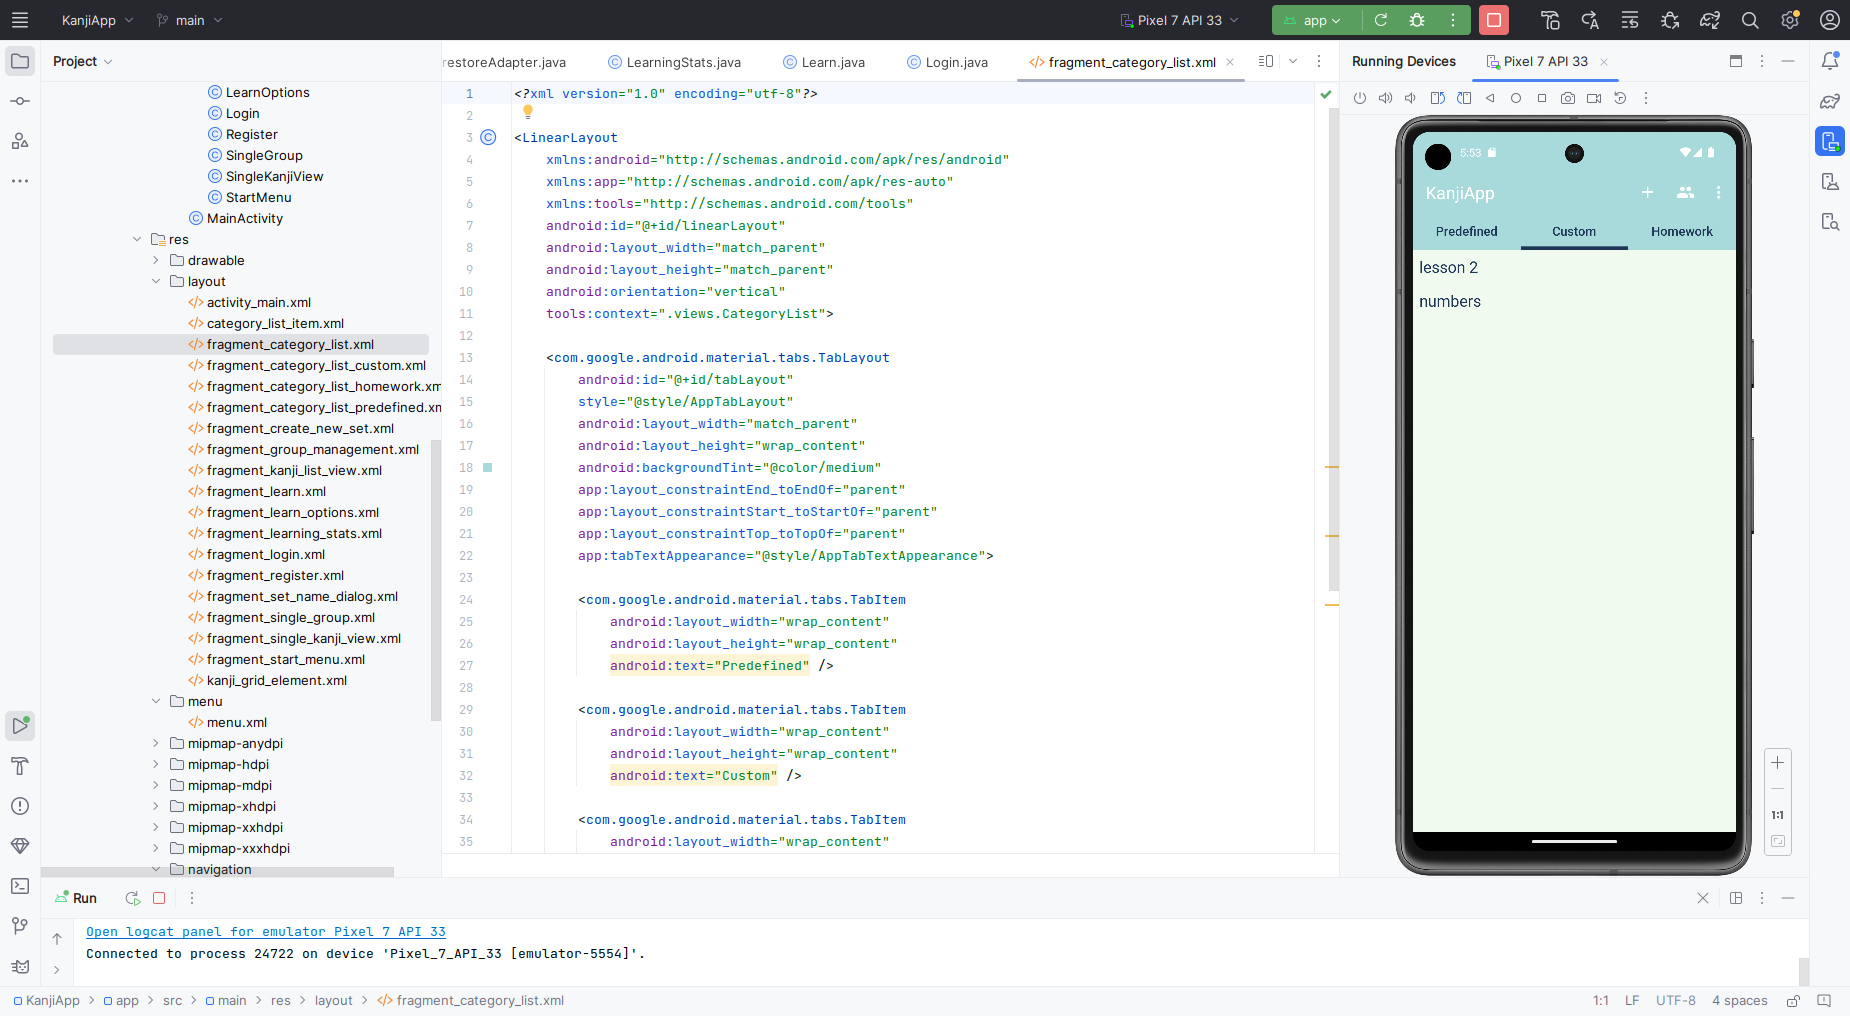
\includegraphics[width=\textwidth]{androidstudio}
\caption{Widok środowiska developerskiego z uruchomionym emulatorem.}
\label{fig:androidstudio}
\end{figure}

Panel administratora został przetestowany z użyciem przeglądarki internetowej Firefox w wersji 120. Angular oferuje pomocne w testowaniu narzędzie wywoływane komendą \texttt{ng serve}, które automatycznie buduje aplikację po każdej zmianie w kodzie, co pozwala na dynamiczną pracę i natychmiastowy widok zmian w interfejsie użytkownika. Innym przydatnym narzędziem było badanie źródła strony w przeglądarce Firefox, które umożliwiło podgląd na konsolę. 

\subsection{Testy automatyczne}

Na potrzeby zautomatyzowanego testowania aplikacji przeznaczonych na system Android można wykorzystać:
\begin{itemize}
\item testy jednostkowe -- testujące pewien fragment kodu taki jak klasa lub metoda,
\item testy integracyjne -- wykorzystujące narzędzia takie jak Robolectric\footnote{\url{https://robolectric.org/}} do testowania większej części kodu lokalnie lub na urządzeniu,
\item testy kompleksowe (ang. \english{end-to-end}) -- symulujące realne używanie aplikacji przez użytkownika za pomocą metod umożliwiających interakcję z interfejsem użytkownika z poziomu kodu.
\end{itemize}

\begin{figure}[]
\centering
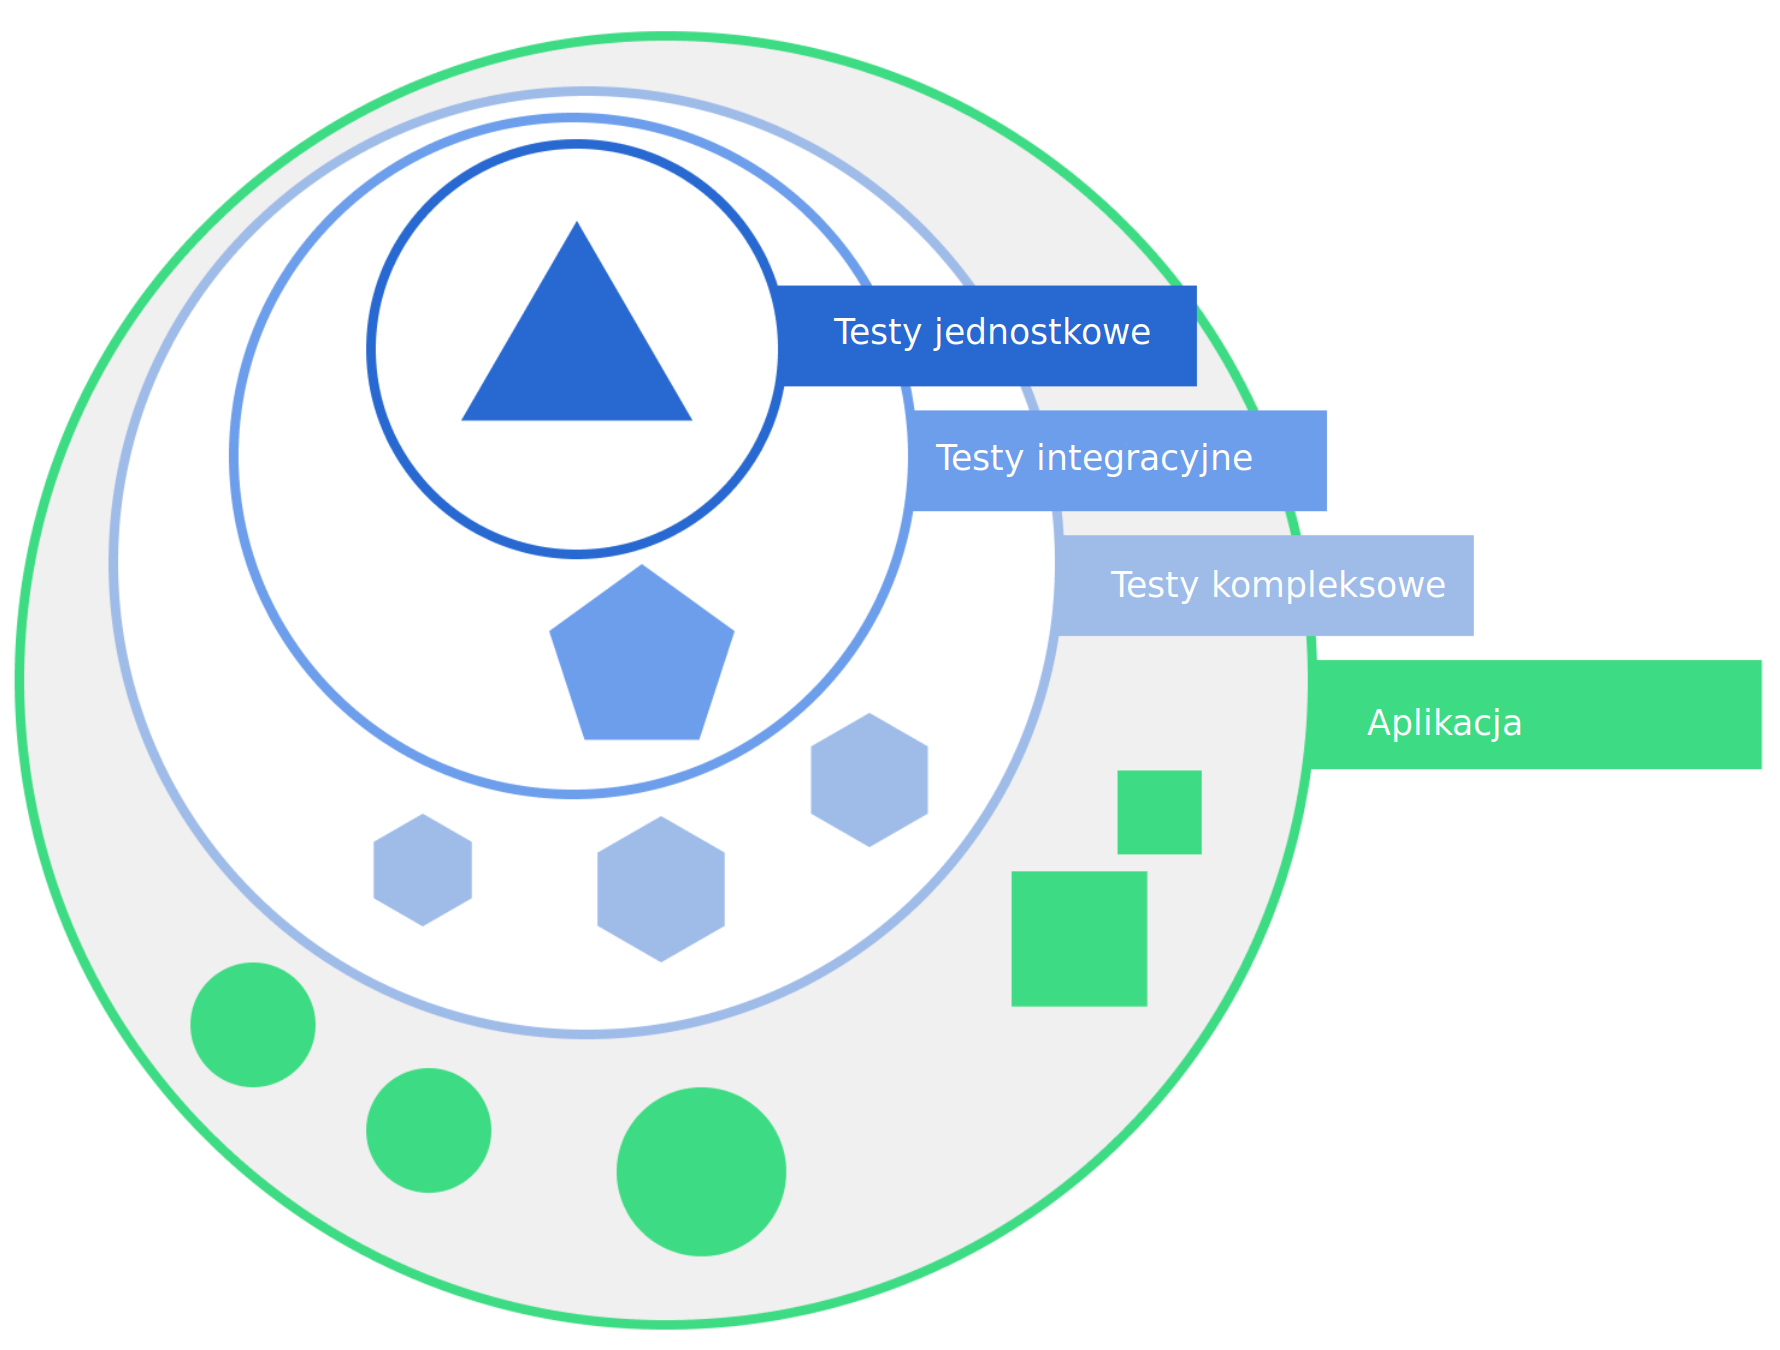
\includegraphics[width=0.7\textwidth]{test-scopes}
\caption{Diagram reprezentujący sposób testowania aplikacji przeznaczonych na system operacyjny Android.}
\label{fig:testscopes}
\end{figure}

Na zakres testowania aplikacji mobilnej opisywanej w tej pracy oprócz testów manualnych składają się testy jednostkowe klas odpowiedzialnych za logikę aplikacji. Aby móc bezpiecznie wydać aplikację na przykład w Sklepie Play, należałoby rozszerzyć testowanie o testy integracyjne i testy interfejsu użytkownika. 

Przykładem klasy przetestowanej za pomocą testów jednostkowych jest \texttt{QuestionGenerator}. Ta klasa jest odpowiedzialna za generowanie pytań (obiektów typu \texttt{QuestionModel}) w sposób, który pozwoli jak najlepiej przyswoić informacje użytkownikowi. Bierze pod uwagę między innymi liczbę odpowiadającą każdemu znakowi, która oznacza biegłość użytkownika w pytaniach dotyczących tego znaku. Na podstawie tych danych generuje losowe pytania dotyczących tych znaków w zestawie, z którymi użytkownik do tej pory radził sobie najgorzej. 

Do przetestowania wyżej opisanej klasy użyto narzędzia Junit\footnote{\url{https://junit.org/junit4/}}, które pozwala na wykonywanie testów jednostkowych. Napisano testy odnoszące się do normalnego trybu działania aplikacji, czyli do tworzenia pytań na podstawie pewnego zestawu znaków. Przetestowano również wpływ błędnych lub nieprzewidywanych danych wejściowych na zachowanie klasy, takich jak wygenerowanie zestawu pytań o liczebności równej zeru. 

\section{Wykryte i usunięte błędy}

%crashe przy uczeniu
Przy testach manualnych aplikacji mobilnej wykryto wiele błędów, większość z nich skutkowała gwałtownym zatrzymaniem działania aplikacji spowodowanym na przykład błędnym odwołaniem do zmiennej lub nieprawidłowym indeksowaniem listy czy tablicy. Takie błędy wynikały z drobnych pomyłek w kodzie i zostały szybko poprawione. Za pomocą testów automatycznych udało się wykryć błąd w klasie odpowiedzialnej za generowanie pytań, która przy przyjęciu błędnie sformatowanego znaku generowała na miejscu pytania wartość \texttt{null}, co powodowało późniejsze gwałtowne zatrzymanie aplikacji.

Przykładowy błąd przy rozwijaniu panelu administratora ujawnił się przy budowaniu aplikacji i umieszczaniu jej na zdalnym serwerze. Przy pierwszych próbach odwiedzenia strony internetowej zawierającej panel administratora wyświetlał się pusty biały ekran. Było to spowodowane błędną konfiguracją przy budowaniu za pomocą Angulara, który używając domyślnej optymalizacji nie współpracował z narzędziami autoryzacji użytkownika Firebase. Problem udało się usunąć dzięki użyciu flagi (\texttt{--optimization=false}) przy budowaniu aplikacji.

% TODO
\chapter{Podsumowanie i wnioski}

%\item uzyskane wyniki w świetle postawionych celów i zdefiniowanych wyżej wymagań
%\item kierunki ewentualnych danych prac (rozbudowa funkcjonalna …)
%\item problemy napotkane w trakcie pracy

%\section{Uzyskane wyniki}

W ramach niniejszej pracy inżynierskiej udało się zbudować aplikację mobilną do nauki znaków kanji oraz strone internetową służącą do administracji. Aplikacja mobilna oferuje możliwość przeglądania słownika znaków według predefiniowanych poziomów trudności oraz nauki owych lub samodzielnie stworzonych zestawów zgodnie z metodą powtórek w interwałach. Dodatkowo, dzięki połączeniu z bazą danych hostowaną w chmurze i serwisem autoryzacji użytkowników Firebase jest możliwość stworzenia konta z uprawnieniami Ucznia bądź złożenia prośby o uprawnienia Nauczyciela, który może tworzyć grupy wspólnej nauki i zadawać im zadania domowe. Kolejny typ użytkownika, czyli Administrator, ma pogląd na listę użytkowników i może zarządzać ich uprawnieniami z poziomu panelu administratora. 

%W trakcie pisania tej pracy udało się zbudować aplikację mobilną do nauki znaków kanji oraz system służący do administracji jej użytkownikami. Wymagania funkcjonalne zostały w większości spełnione, jednak pozostało kilka elementów które zostały pominięte na rzecz ważniejszych zadań, których nie udało się przewidzieć na początku planowania pracy. \ksremark{$\gets$ nie tak. Tutaj piszemy, jakie ma cechy aplikacja. Czyli coś w stylu: W ramach niniejszej pracy inżynierskiej powstała aplikacja taka i siaka. Aplikacja umożliwia, no i tu piszemy, jaka jest jej funkcjonalność.} Najważniejsze cechy aplikacji, czyli możliwość przeglądania słownika znaków oraz nauka z użyciem metody powtórek w interwałach zostały zaimplementowane. Pominięto takie funkcjonalności jak nauka pisania poprzez rysowanie na telefonie lub informacja zwrotna dla nauczyciela zadającego zadanie domowe. Aplikacja jest otwarta na modyfikacje, w przyszłości więc jest możliwość dodania wyżej wymienionych przypadków użycia. Rozwiązanie spełnia założenia wymagań niefunkcjonalnych za wyjątkiem nieco większego pliku lokalnie przechowywanej bazy danych niż zakładano.

Aplikacja do nauki znaków kanji ma duży potencjał na rozwój jej funkcjonalności. Nauka badająca sposoby, w jakie ludzie zapamiętują nowe informacje, szczególnie w kontekście języków obcych nauczanych komputerowo może przynieść wiele inspiracji do udoskonalania algorytmu dostarczającego zadania do użytkownika. Dodatkowo można znacznie ulepszyć działanie aplikacji z programistycznego punktu widzenia, na przykład wykonać refraktoryzację kodu na wzorzec projektowy MVP lub zaprojektować bardziej intuicyjny interfejs użytkownika.

Często występującym problemem w dziedzinie komputerowo wspomaganego nauczania języków jest binarne postrzeganie problemu przez komputer. Jeśli sprawdzanie poprawności odpowiedzi odbywa się po prostu za pomocą porównania łańcuchów znaków, wszystkie nieszablonowe lub zawierające drobne literówki odpowiedzi będą traktowane jako niepoprawne. Przy takim podejściu nie ma możliwości przyznania części punktu, jak to odbywa się w tradycyjnym nauczaniu. Implementując inteligentniejszy system sprawdzania odpowiedzi można też zauważyć pewnie tendencje użytkownika i wykorzystać tą wiedzę do dostosowania strategii nauczania. Przy takich zadaniach mogą się okazać pomocne technologie przetwarzania języka naturalnego (ang. \english{natural language processing, NLP}).

Dużym obszarem, w którym aplikacja mobilna mogłaby się rozwinąć jest testowanie. Zaczynając od pokrycia testami jednostkowymi całego kodu, przez testy integracyjne aż do testów interfejsu użytkownika -- dzięki kompleksowemu testowaniu aplikacja mogłaby dużo zyskać na stabilności i bezpieczeństwie. W dalszych etapach rozwoju można by też rozważyć wykorzystanie praktyk ciągłej integracji i ciągłego wdrażania.

Kod źródłowy rozwiązania jest dostępny na repozytorium w serwisie GitHub\footnote{\url{https://github.com/aleksandrakyc/kanji-learning-app}}, a panel administratora można odwiedzić na stronie internetowej\footnote{\url{https://kanjilearningapp-e002b.web.app/}}.
\backmatter

%\bibliographystyle{plplain}  % bibtex
%\bibliography{biblio} % bibtex
\printbibliography           % biblatex
\addcontentsline{toc}{chapter}{Bibliografia} 
\begin{appendices}
% TODO
\chapter{Spis skrótów i symboli}



% TODO
\chapter{Źródła}



% % % % % % % % % % % % % % % % % % % % % % % % % % % % % % % % % % % 
% Pakiet minted wymaga odkomentowania w pliku config/settings.tex   %
% importu pakietu minted: \usepackage{minted}                       %
% i specjalnego kompilowania:                                       %
% pdflatex -shell-escape praca                                      %
% % % % % % % % % % % % % % % % % % % % % % % % % % % % % % % % % % % 

%\begin{minted}[linenos,breaklines,frame=lines]{c++}
%if (_nClusters < 1)
%   throw std::string ("unknown number of clusters");
%if (_nIterations < 1 and _epsilon < 0)
%   throw std::string ("You should set a maximal number of iteration or minimal difference -- epsilon.");
%if (_nIterations > 0 and _epsilon > 0)
%   throw std::string ("Both number of iterations and minimal epsilon set -- you should set either number of iterations or minimal epsilon.");
%\end{minted}


% TODO
\chapter{Lista dodatkowych plików, uzupełniających tekst pracy} 


W systemie do pracy dołączono dodatkowe pliki zawierające:
\begin{itemize}
\item źródła programu,
\item dane testowe,
\item film pokazujący działanie opracowanego oprogramowania lub zaprojektowanego i~wykonanego urządzenia,
\item itp.
\end{itemize}


\listoffigures
\addcontentsline{toc}{chapter}{Spis rysunków}
\listoftables
\addcontentsline{toc}{chapter}{Spis tabel}

\end{appendices}

\end{document}


%% Finis coronat opus.

